\documentclass[12pt]{article}
\usepackage{placeins}
\usepackage{hcmus-report-template}

% Disable indentation on new paragraphs
\setlength{\parindent}{0pt}

% Line spacing 1.5
\renewcommand{\baselinestretch}{1.5}

% Optional: graphic path
% \graphicspath{PATH_TO_GRAPHIC_FOLDER}

% To use Times font family, uncomment this row
% \usepackage{mathptmx}

% To use roman section / subsection, uncomment these rows
% \renewcommand{\thesection}{\Roman{section}}
% \renewcommand{\thesubsection}{\thesection.\Roman{subsection}}

% Define course name, report name and report title.
\newcommand{\coursename}{CS202 -- Programming Systems}
\newcommand{\reportname}{Mario 2D Game}
\newcommand{\reporttitle}{Mario Game Project Report}

\newcommand{\studentname}{
\begin{itemize}
    \item Tran Minh Khoa -- 25125057
    \item Tran Nhu Khai -- 25125045
    \item Do Viet Hoang Long -- 25125024
    \item Tran Dang Khoa -- 25125056
\end{itemize}
}

% Header
\lhead{\reporttitle}
\rhead{
CS202 -- Group 3
}


% ============ DOCUMENT ============
\begin{document}

\pagenumbering{arabic}
\begin{titlepage}
\newcommand{\HRule}{\rule{\linewidth}{0.5mm}}
\centering

% ===== UNIVERSITY =====
\textsc{\LARGE Vietnam National University - HCMC}\\[0.5cm]
\textsc{\Large University of Science}\\[0.5cm]
\textsc{\large Faculty of Information Technology}\\[0.5cm]

\vspace{0.5cm}
\HRule \\[1.0cm]

% ===== TITLE =====
{\huge \bfseries \reporttitle}\\[0.5cm]

\HRule \\[1.0cm]

% ===== COURSE =====
{\large \textbf{Course: \coursename}}\\[1.0cm]

% ===== STUDENT & INSTRUCTOR =====
\begin{flushleft} \large
\emph{Students:}\\
\studentname
\end{flushleft}

\begin{center}
    
\includegraphics[scale=0.25]{img/hcmus-logo.png}
\end{center}

% ===== DATE =====
{\large August, 2026}

\vfill
\end{titlepage}

\tableofcontents
\section{Abstract}
The Mario Game Project is a two-dimensional platform game developed in C++ using the SFML multimedia library. Inspired by classic side-scrolling platformers, the project combines character movement, combat, power-up transformations, enemy artificial intelligence, collision detection, interactive environments, and level progression within a custom game architecture. Players can choose from multiple heroes—including Mario, Luigi, and Flash—each with distinct visual styles and special abilities. The game implements several character forms, collectible items, destructible blocks, projectile mechanics, pipe travel, configurable audio, HUD management, and specialized enemies such as Goomba, Koopa, Witch, and the multi-phase boss. Object-oriented design principles and behavioral patterns are used to separate game states, character forms, animations, physics, interactions, and level management. The project also introduces JSON-based save and load functionality for retaining essential gameplay progress. Overall, the system demonstrates how modular software design can support an extensible platform game while maintaining clear responsibilities between gameplay, presentation, and data-management components.

\section{Introduction}
Two-dimensional platform games provide a useful environment for studying game development because they combine real-time input, animation, physics, collision detection, artificial intelligence, resource management, and user-interface design. Although their basic objective is easy to understand, implementing a reliable platform game requires many interconnected systems to operate consistently. Character movement must respond smoothly to player input, collisions must be resolved without allowing entities to pass through the environment, enemies must react appropriately, and visual animations must remain synchronized with the underlying gameplay state.

The Mario Game Project was developed as a custom C++ platform game inspired by the mechanics of the Super Mario series. The game allows players to control Mario, Luigi, or Flash. Each hero shares a common movement and interaction framework while providing different textures, animations, and projectile-based special abilities. Heroes can collect mushrooms to enter a larger form and flowers to unlock an advanced form, such as Fire Mario or ThunderFlash. Other gameplay elements include collectible coins, temporary invincibility, interactive blocks, pipes, environmental obstacles, and multiple enemy types.

A major objective of the project is to apply object-oriented programming principles to a practical game system. Common entity behavior is represented through inheritance and polymorphism, while specialized classes implement the unique behavior of heroes, enemies, items, blocks, and projectiles. Character forms and movement conditions are modeled using separate form and state classes. This approach allows transitions such as growing, shrinking, jumping, crouching, taking damage, and celebrating victory to be managed without placing all behavior inside a single character class. Factory classes are also used to create heroes, enemies, blocks, and items from level data.

The project separates the gameplay world from presentation and application-level state management. Dedicated systems handle physics, entity interactions, level construction, runtime updates, animation, sound, HUD information, menus, pause behavior, victory, defeat, and transitions between screens. Levels are loaded from Tiled map files, enabling terrain, triggers, enemy spawners, interactive objects, pipe routes, and goal regions to be configured outside the source code. A JSON-based save mechanism records important information such as the active level, hero status, enemy data, modified blocks, score, coins, lives, and remaining time.

This report presents the design and implementation of the Mario Game Project, with particular attention to its software architecture, gameplay systems, object-oriented design, enemy behavior, physics, animation, user interface, and persistence mechanism. It also discusses integration challenges encountered during development and identifies areas for future improvement.
\section{Group Information}
\subsection{Team Roles and Contributions}

The project was developed collaboratively, with each member responsible for a specific data structure or system component. In addition to their core responsibilities, members also contributed to integration, testing, and ensuring consistency across the system.

\subsubsection{Tran Minh Khoa}

\textbf{Role:} Core Engine \& Physics \\
\textbf{Responsibilities:}
\begin{itemize}
    \item Manage the SFML RenderWindow, Game Loop, and Game States.
    \item Implement precise AABB collision detection.
    \item Apply gravity and physics.
\end{itemize}

\subsubsection{Tran Nhu Khai}

\textbf{Role:} Hero \& Items Mechanics \\
\textbf{Responsibilities:}
\begin{itemize}
    \item Lead the project and design the initial workflow of the project.
    \item Build the base \texttt{Character} class and the \texttt{Mario} class (and other Character class).
    \item Implement classic items (Mushroom, Coin, Fire Flower) using the Factory Pattern.
\end{itemize}

\subsubsection{Do Viet Hoang Long}

\textbf{Role:} Enemies \& AI \\
\textbf{Responsibilities:}
\begin{itemize}
    \item Inherit the \texttt{Character} class to create the base \texttt{Enemy} abstract class.
    \item Create classic enemies (Goombas, Koopas).
    \item Implement standard patrol AI using the Template Method.
\end{itemize}

\subsubsection{Tran Dang Khoa}

\textbf{Role:} Level, UI/UX \& Audio \\
\textbf{Responsibilities:}
\begin{itemize}
    \item Build a Map Parser to load classic Mario levels from text/csv files.
    \item Implement the HUD (score, coins, lives) via the Observer Pattern.
    \item Develop a SoundManager for 8-bit BGM and SFX.
\end{itemize}

\subsection{Overall Contribution}
The Mario game project was completed through close collaboration among all team members, with each person taking responsibility for a major gameplay system and then integrating their work into a unified project. Tran Minh Khoa focused on the core engine and physics aspects, including the render loop, collision handling, and gravity-based movement. Tran Nhu Khai developed the main character and item mechanics, constructing the base character hierarchy and implementing collectible items using a factory-based design. Do Viet Hoang Long handled enemies and AI by creating the enemy structure and basic patrol behaviors. Tran Dang Khoa designed the level system, HUD, and sound management, enabling stage loading, game status display, and audio feedback.

Across the whole project, all members participated in debugging, testing, and refining the game to ensure stable gameplay, correct interactions, and smooth project integration. This division of responsibility allowed the team to build a complete and coherent Mario-style game while maintaining code organization and reusability.

\subsection{Commit List (Git History) - brief version}

It has been refined and condensed for easier reading compared to the original text from \texttt{git log}.

Or  on gitHub:
\href{https://github.com/trannhukhai98438/CS202-Group03-2DGame.git}{
    \boxed{Click\;  here}
}
\section{Project Design}
% Include class diagrams and reasonings of the design
\label{sec:project-design}
\begingroup
\sloppy

\subsection{Scope and Architectural Objectives}

The Mario Game Project is a C++17, SFML-based two-dimensional platformer.  It
supports three selectable heroes, three selectable levels, data-driven Tiled
maps, multiple hero forms, enemy AI, a multi-phase boss, blocks and power-ups,
hero and enemy projectiles, sound, a HUD, pause/save/continue flows, and victory
or defeat transitions.  The design has four primary objectives:

\begin{enumerate}
    \item keep application navigation separate from gameplay simulation;
    \item construct levels and entities from map or save data rather than in
    the main loop;
    \item represent behavior through polymorphism and composition so new
    characters, states, entities, and levels can be added locally; and
    \item make ownership explicit through RAII smart pointers, with narrow
    non-owning callbacks for cross-system events.
\end{enumerate}

The implementation is organized into the \texttt{Core}, \texttt{Gameplay},
\texttt{Entities}, \texttt{Managers}, and \texttt{Utilities} areas.  SFML
provides the window, events, timing, graphics, views, textures, text, and audio.
Tiled \texttt{.tmj} maps are parsed with the vendored nlohmann JSON library.

\subsection{High-Level Architecture}

At the highest level, \texttt{Game} runs a fixed-step application state stack.
\texttt{PlayingState} is the presentation-level controller for an active game,
while \texttt{LevelRuntime} is the gameplay facade.  The latter owns the world
and delegates physical movement and entity interactions to dedicated systems.

\begin{figure}[htbp]
\centering
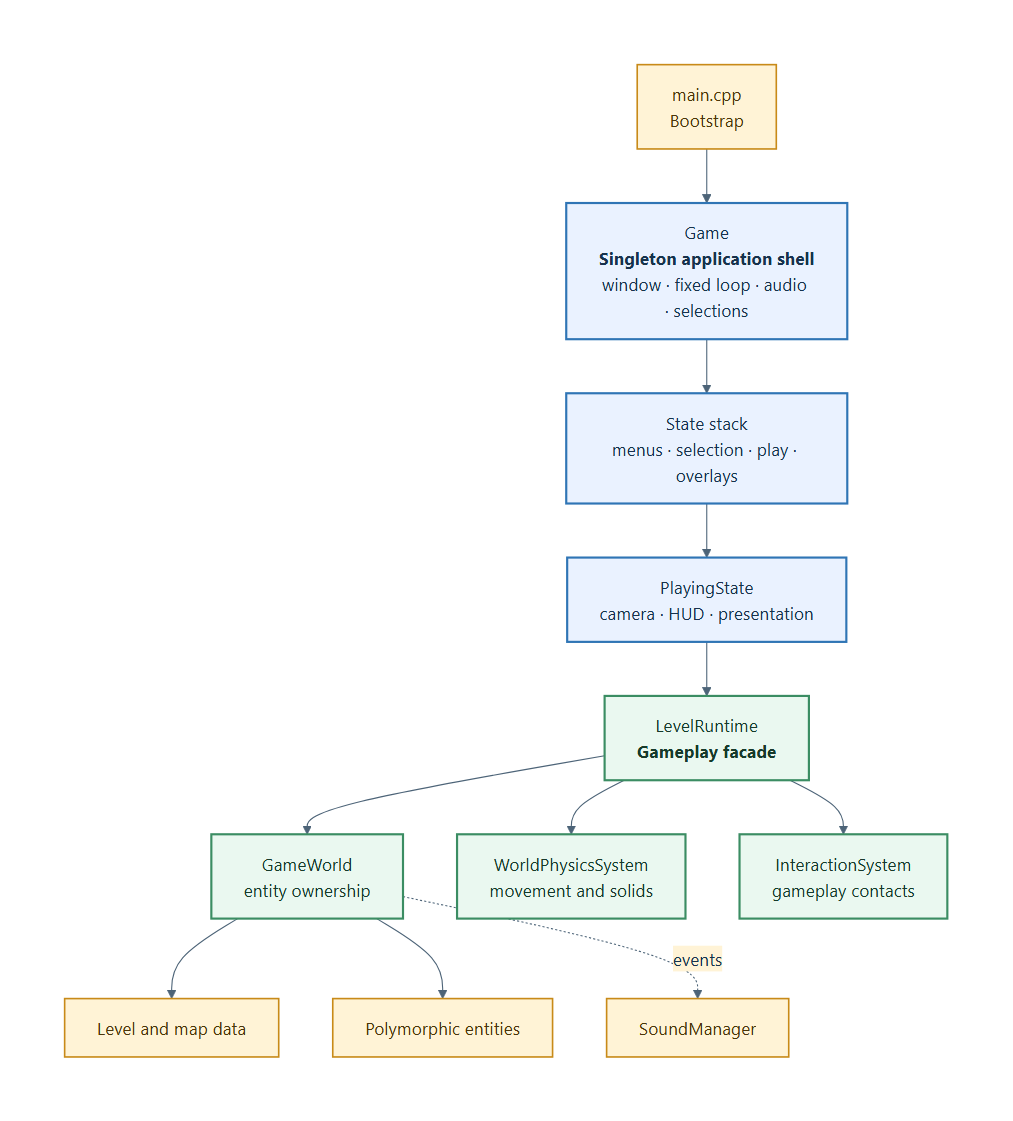
\includegraphics[width=0.76\textwidth,height=0.68\textheight,keepaspectratio]{img/diagrams/project-overall-architecture.png}
\caption{Layered runtime architecture of the game.}
\label{fig:overall-architecture}
\end{figure}

\begin{table}[htbp]
\centering
\small
\renewcommand{\arraystretch}{1.2}
\begin{tabular}{|p{0.19\textwidth}|p{0.33\textwidth}|p{0.37\textwidth}|}
\hline
\textbf{Area} & \textbf{Main abstractions} & \textbf{Responsibility} \\
\hline
Application shell & \texttt{Game}, \texttt{State} and concrete screen states & Window and fixed loop, event dispatch, screen navigation, overlays, global selection and audio lifetime. \\
\hline
Gameplay facade & \texttt{PlayingState}, \texttt{LevelRuntime} & Camera/HUD and transitions on one side; ordered simulation and region/pipe behavior on the other. \\
\hline
World and systems & \texttt{GameWorld}, \texttt{LevelBuilder}, \texttt{WorldPhysicsSystem}, \texttt{InteractionSystem} & Entity ownership, initial construction, terrain collision, entity-to-entity rules, and cleanup. \\
\hline
Domain entities & Characters, blocks, items, projectiles, goals & Polymorphic gameplay behavior and rendering. \\
\hline
Data/services & Map, level, save, HUD and sound managers & Parse and render map data, persist sessions, display metrics, and play audio. \\
\hline
Utilities & \texttt{Animator}, physics constants, shared Thunder Flash texture & Reusable animation, tuning constants, and lazy texture processing. \\
\hline
\end{tabular}
\caption{Primary architectural areas and responsibilities.}
\end{table}

\subsection{Overall Class Diagram}
\label{subsec:overall-class-diagram}

Figure~\ref{fig:overall-class-diagram} summarizes the main static relationships
across the complete project.  The application layer owns polymorphic screen
states and long-lived services.  The active \texttt{PlayingState} owns one
\texttt{LevelRuntime}, which acts as the facade over world data, physics, and
semantic interactions.  \texttt{GameWorld} is the aggregate root for live
entities, while heroes and enemies delegate their changing behavior to form and
state objects.  Builders and managers remain outside the entity hierarchies so
that construction, persistence, and presentation do not become entity concerns.

\begin{figure}[p]
\centering
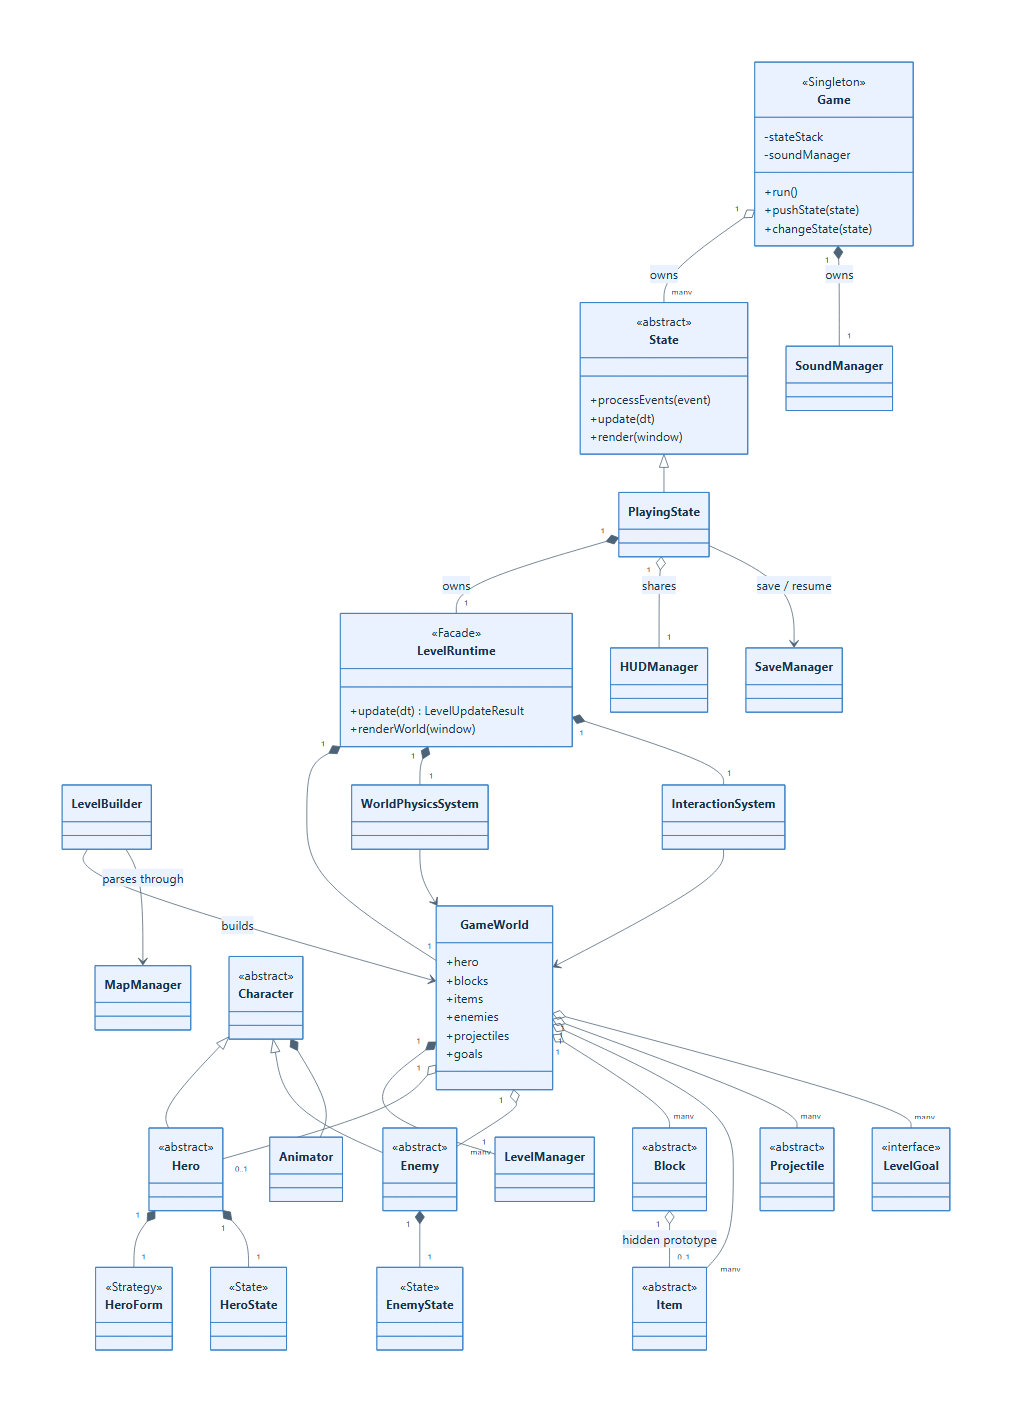
\includegraphics[width=0.94\textwidth,height=0.82\textheight,keepaspectratio]{img/diagrams/project-overall-class.png}
\caption{Overall class diagram of the application shell, gameplay facade,
world ownership, domain entities, and supporting services.}
\label{fig:overall-class-diagram}
\end{figure}

The diagram deliberately shows architectural classes and families rather than
every concrete subclass.  The focused diagrams in the following subsections
expand the screen, hero, enemy, block, item, projectile, goal, and service areas.

\subsection{Application Bootstrap, Main Loop, and State Stack}

\subsubsection{Bootstrap and resource lifetime}

\texttt{src/main.cpp} is intentionally small.  It obtains the singleton
\texttt{Game}, queues a \texttt{MainMenuState}, and calls \texttt{run()}.
\texttt{Game} owns the only \texttt{sf::RenderWindow}, the state stack, the
long-lived \texttt{SoundManager}, selected hero and level metadata, and global
volume settings.  On Windows, \texttt{main.cpp} also contains a compatibility
definition for legacy standard-I/O symbols required by the linked environment.

The loop uses a fixed simulation step of $1/60$ second and a variable render
rate.  Elapsed wall time is clamped to $0.25$ seconds before it is accumulated.
This cap is important when a large map or texture takes time to load: the game
does not spend many seconds replaying accumulated fixed updates after the load.
Events are polled during fixed updates, the active state is updated, and the
visible portion of the state stack is rendered once per outer loop iteration.

State transitions are deferred.  A state may request Push, Pop, Replace, or
Clear-and-Push, but \texttt{Game::applyPendingStateAction} commits the request
outside the state's callback.  This prevents deletion of a state while its own
event or update function is executing.  Repeated Tab and Enter key-press events
are filtered until their key-release events, preventing duplicate activations.

\subsubsection{Screen-state class diagram}

\begin{figure}[htbp]
\centering
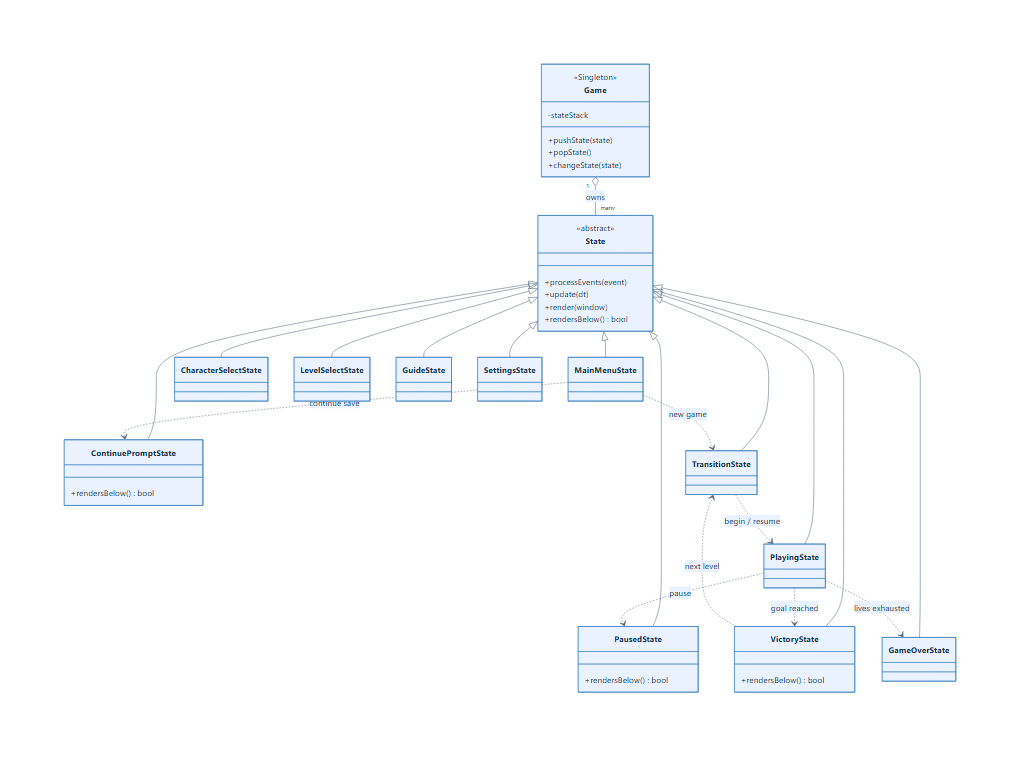
\includegraphics[width=0.98\textwidth,height=0.68\textheight,keepaspectratio]{img/diagrams/project-screen-states.png}
\caption{Application state hierarchy and principal navigation paths.}
\label{fig:screen-state-diagram}
\end{figure}

\subsubsection{Responsibilities of each screen}

\begin{description}
    \item[\texttt{MainMenuState}] Presents Play, Character, Level, Guide, and
    Settings buttons.  Play opens \texttt{ContinuePromptState} if an existing
    save is found; otherwise it starts a transition directly.  The menu also
    displays the currently selected world and starts menu background music.

    \item[\texttt{ContinuePromptState}] Is a modal overlay
    (\texttt{rendersBelow()} is true).  It validates the save's map and tileset,
    resolves its catalog/world labels, and offers Continue or New Game.
    Continuing restores HUD metadata and enters \texttt{TransitionState} with
    a resume flag; New Game clears the stack and uses current selections.

    \item[\texttt{CharacterSelectState}] Displays Mario, Luigi, and Flash cards.
    Confirmation writes a \texttt{HeroType} into \texttt{Game} and returns to
    the menu.  It does not construct the hero; construction is deferred until
    a level is built.

    \item[\texttt{LevelSelectState}] Builds its three cards from
    \texttt{LevelCatalog::LEVELS}.  Levels 1, 2, and 3 correspond to worlds
    1-1, 1-2, and 1-3 and are currently marked \texttt{READY}.  Confirmation
    stores the map path and world label in \texttt{Game}.

    \item[\texttt{GuideState}] Implements a paged help screen with character,
    item, and keyboard/control illustrations.

    \item[\texttt{SettingsState}] Owns two reusable slider records for BGM and
    SFX volume.  Keyboard, mouse, hover, and drag operations update the global
    \texttt{Game} settings and therefore the live \texttt{SoundManager}.

    \item[\texttt{TransitionState}] Displays the selected world and remaining
    lives for two seconds, then replaces itself with \texttt{PlayingState}.  A
    shared \texttt{HUDManager} survives retries and next-level transitions.

    \item[\texttt{PlayingState}] Owns camera and HUD presentation, one
    \texttt{LevelRuntime}, pause/save integration, level theme music, victory
    and defeat delays, and Thor King phase-three environmental effects.

    \item[\texttt{PausedState}] Is a modal overlay containing Resume, Save, and
    Main Menu commands.  The Save command invokes a callback supplied by the
    underlying \texttt{PlayingState}; the pause state therefore does not need
    access to the complete world.

    \item[\texttt{VictoryState}] Is a modal animated overlay offering Replay,
    Main Menu, and Next Level.  Next Level uses
    \texttt{LevelCatalog::nextAfter}, preserves the shared HUD, resets the
    timer, updates the selected level, and enters another transition.

    \item[\texttt{GameOverState}] Presents the defeat animation and returns to
    the menu when Enter is pressed.
\end{description}

This state hierarchy is preferable to a single screen-mode switch in the main
loop.  Every screen owns only its own graphical controls and input rules, while
\texttt{Game} supplies one uniform lifetime and navigation protocol.

\subsection{Gameplay Coordination and World Ownership}

\subsubsection{Facade and subsystem boundaries}

\texttt{PlayingState} is intentionally not the owner of entity collections.
It delegates them to \texttt{LevelRuntime}, which provides a facade over the
complete running level.  \texttt{LevelRuntime} in turn owns
\texttt{GameWorld}, \texttt{WorldPhysicsSystem}, and
\texttt{InteractionSystem}; it creates a short-lived \texttt{LevelBuilder} for
initial construction or reload.

\begin{figure}[htbp]
\centering
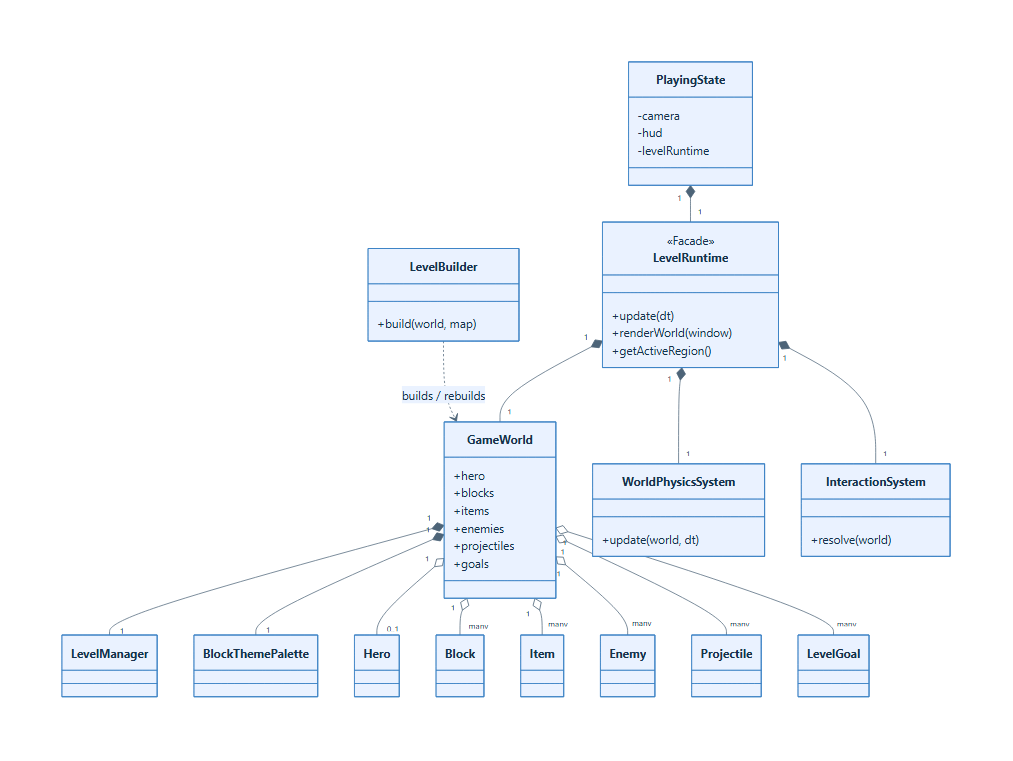
\includegraphics[width=0.95\textwidth,height=0.68\textheight,keepaspectratio]{img/diagrams/project-gameplay-facade.png}
\caption{Gameplay facade, systems, and ownership.}
\label{fig:gameplay-facade-diagram}
\end{figure}

\texttt{GameWorld} is the aggregate root for live gameplay data.  Its entity
collections use \texttt{std::unique\_ptr}; consequently, an entity has exactly
one owner and is destroyed automatically when removed or when the world is
cleared.  Systems receive a \texttt{GameWorld\&} temporarily and never take
ownership.  \texttt{SoundManager*} is explicitly non-owning because the audio
service belongs to \texttt{Game} and outlives every level.

\texttt{GameWorld::removeInactiveEntities} is the deferred cleanup point.
Entities mark themselves inactive, collected, or dead during update and
interaction passes; erasure occurs afterward, avoiding iterator invalidation.
For destroyed map blocks, the world also retains tile-coordinate pairs used by
persistence.  The world exposes a map-collider collection built from terrain
tiles for compatibility, while current high-frequency physics queries use the
\texttt{LevelManager} tile grid directly.

\subsubsection{Per-frame update order}

The order of a frame is part of the game's behavior:

\begin{enumerate}
    \item \texttt{PlayingState} obtains a newly pressed pipe direction and
    calls \texttt{LevelRuntime::update}.
    \item The runtime snapshots the room-bottom boundary of each active enemy.
    This prevents an enemy falling from a vertically stacked room from being
    incorrectly reassigned to the room below.
    \item Intrinsic updates run in the order Hero, Blocks, Items, Enemies, and
    Projectiles.  These updates handle input, state changes, animation,
    acceleration policy, timers, and spawning intent.
    \item \texttt{WorldPhysicsSystem} integrates velocity and resolves terrain
    and block collisions.
    \item \texttt{InteractionSystem} resolves cross-entity contacts and returns
    one score delta.
    \item The runtime enforces the live boss-arena boundary, attempts pipe
    travel, synchronizes the active region, applies hero/enemy fall deaths,
    culls out-of-world projectiles, and removes inactive entities.
    \item Back in \texttt{PlayingState}, score and coin changes are applied to
    the HUD; theme or invincibility music and the pixel-aligned camera are
    updated; then victory, time-out, defeat, and boss VFX are processed.
\end{enumerate}

Victory becomes authoritative once a goal has activated.  The hero enters
\texttt{CheerState}; after a short delay, a \texttt{VictoryState} overlay is
pushed.  Defeat restores the score/coin/lives snapshot from the start of the
attempt, removes one life, plays the player-down cue, and after two seconds
either retries through \texttt{TransitionState} or enters
\texttt{GameOverState}.

\subsubsection{Rendering order}

\texttt{PlayingState} installs the world camera and draws an underground black
backdrop when appropriate.  \texttt{LevelRuntime::renderWorld} then draws the
tile-map mesh, blocks in the active region, items, hero, enemies, and
projectiles.  Thor King phase-three overlays, lightning, fissures, and debris
are drawn by \texttt{PlayingState}.  Finally, the HUD is drawn in the default
window view so it remains screen-relative, and the default view is restored.

\subsection{Level and Map System}

\subsubsection{Data model and loading pipeline}

The level pipeline deliberately separates parsing, storage, rendering, and
gameplay construction.

\begin{figure}[htbp]
\centering
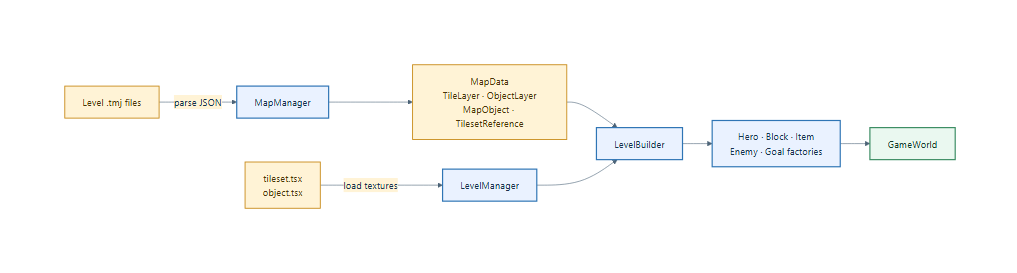
\includegraphics[width=0.96\textwidth,height=0.48\textheight,keepaspectratio]{img/diagrams/project-level-pipeline.png}
\caption{Data-driven level loading and construction pipeline.}
\label{fig:level-pipeline-diagram}
\end{figure}

\texttt{MapManager} parses map dimensions, tile size, tileset references,
visible tile layers, object layers, Tiled's modern \texttt{class} field with a
legacy \texttt{type} fallback, geometry, GIDs, and scalar custom properties.
\texttt{MapObject} retains all scalar properties in a string map and also
populates typed aliases such as target map, direction, contained item, theme,
and count.  \texttt{MapData} provides layer lookup, class queries, map pixel
dimensions, and matching pipe exits.

\texttt{LevelManager} owns the parsed \texttt{MapData}, the main and optional
object textures, and one pair of \texttt{sf::VertexArray} meshes per visible
tile layer.  At load time it resolves TSX image paths and converts all non-empty
tiles into texture-mapped quads.  Main-atlas and object-atlas quads are batched
separately, which reduces per-frame draw work compared with one sprite per tile.
It also supplies tile ID, solid-at-tile/pixel, interactive-tile, tile mutation,
and flexible object-query operations.  Pixel art uses nearest-neighbor sampling
and non-repeating textures to prevent atlas bleeding.

\subsubsection{Level construction}

\texttt{LevelBuilder::build} performs these steps:

\begin{enumerate}
    \item load the map and tilesets through \texttt{LevelManager};
    \item create the callback through which heroes and enemies transfer new
    projectiles into \texttt{GameWorld};
    \item find \texttt{Trigger/start} (with a legacy spawn fallback), create the
    selected hero through \texttt{HeroFactory}, and interpret the Tiled point as
    a foot-position anchor;
    \item create terrain rectangles for solid tiles;
    \item create Flag or Princess goal triggers from \texttt{Trigger/end};
    \item translate \texttt{Interactive} objects into bricks, question blocks,
    invisible blocks, ground coins, or a fallback flag, using factories and
    contained-item properties;
    \item match platform-up/platform-down spawners to unique
    \texttt{platform\_despawn} boundaries and construct \texttt{Lifter}
    platforms; and
    \item translate other \texttt{Spawner} objects into Goombas, Koopas,
    Witches, or Thor King.  Boss sound events are connected to the audio service.
\end{enumerate}

The construction code accepts selected legacy/case variants of object classes,
which protects existing maps during schema evolution.  New map schemas should
prefer one canonical spelling to reduce string-based branching.

\subsubsection{Playable regions, themes, pipes, and boss arena}

\texttt{LevelRuntime} caches valid \texttt{Trigger/playable\_region} rectangles.
The active region supplies the fall boundary, vertical camera anchor, block
theme, and block-render visibility.  Direct movement may switch between
side-by-side regions with vertical overlap; vertically stacked rooms are
switched explicitly through pipe destinations so falling into a pit cannot
accidentally enter the room below.  If no unique region contains the hero, the
runtime uses full map bounds and can infer a fallback theme from a boss arena.

Pipe entrances are \texttt{pipe\_in} triggers whose names match
\texttt{pipe\_out} objects.  Direction, hero alignment, grounded state, allowed
movement state, destination region, and a short cooldown are all checked.  The
destination point is interpreted as center-X and feet-Y, which keeps different
hero forms aligned.  The input direction is latched until release so a held key
does not immediately travel back through the exit.

Level 1-3 contains the current boss area.  A \texttt{boss\_arena} trigger gives
the arena metadata, and a boss spawner produces \texttt{ThorKing}.  While the
boss is alive, the runtime clamps the hero against the configured arena edge;
the restriction disappears after the boss dies.  The Princess goal represents
the final rescue endpoint.

\subsubsection{Current level catalogue}

\texttt{LevelCatalog.h} is a compile-time catalogue containing the displayed
number, world name, readiness status, map path, transition title, and compact
HUD world label for each level.  World 1-1 is an overworld with an underground
pipe room; world 1-2 is a larger multi-region level with several paired pipes
and moving lifters; world 1-3 is the boss level with Witches, Thor King, and a
Princess goal.  The associated data files are
\texttt{assets/maps/levels/1-1.tmj},
\texttt{assets/maps/levels/1-2.tmj}, and
\texttt{assets/maps/levels/1-3.tmj}; shared Tiled definitions are
\texttt{assets/maps/resources/tileset.tsx} and
\texttt{assets/maps/resources/object.tsx}.

\subsection{Character and Hero System}

\subsubsection{Base character abstraction}

\texttt{Character} is the abstract root for heroes and enemies.  It centralizes
position, velocity, hitbox shape, sprite, owned texture, animation controller,
life, facing direction, and grounded state.  Its polymorphic contract includes
update, render, damage, interaction, stomp/side-collision responses, speed,
health, touch damage, score value, and a stable type name.  The common setters
keep logical position, hitbox, and sprite synchronized.

\subsubsection{Hero class diagram}

\begin{figure}[htbp]
\centering
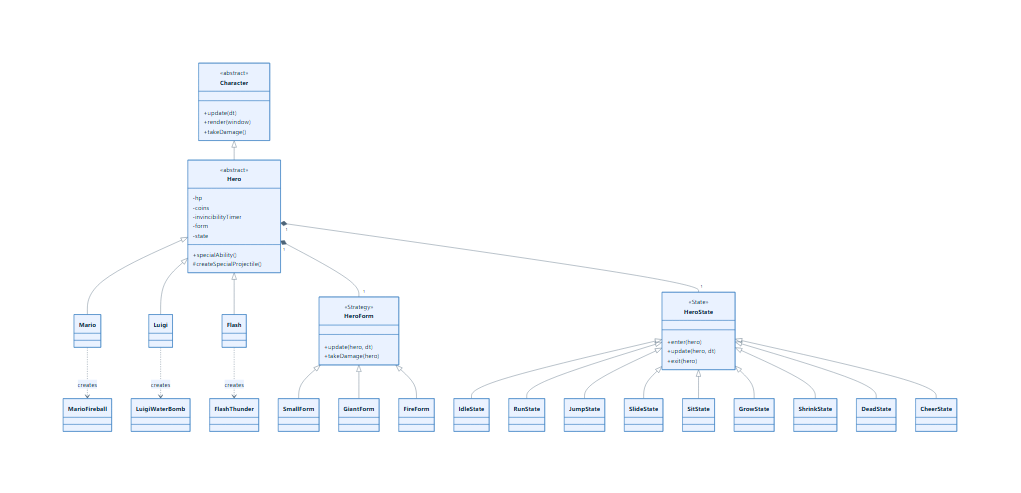
\includegraphics[width=0.99\textwidth,height=0.58\textheight,keepaspectratio]{img/diagrams/project-hero.png}
\caption{Character inheritance and the two orthogonal hero behavior axes.}
\label{fig:hero-class-diagram}
\end{figure}

\texttt{Hero} adds a form strategy, a movement state, base and special texture
paths, form-dependent sprite scales, override animation, invincibility and
Starman timers, coin and HP data, projectile spawning, and SFX callbacks.
\texttt{Hero::update} updates timers, synchronizes coordinates, delegates to
the form and state, and composes an animation key from form plus state (for
example, \texttt{GiantRun}).  Override animation supports a temporary special
attack without replacing the movement state.

Damage is form-dependent.  Small form dies, Giant form enters a Shrink state,
and Fire form first downgrades to Giant before using Giant's shrink behavior.
Invincibility frames prevent duplicate damage and render as blinking; Starman
invincibility uses color cycling and special music.  A falling hero who meets
the top portion of an enemy invokes \texttt{onStomped}, bounces upward, and
returns the enemy's score; other contact delegates to the enemy's side-collision
policy.

\subsubsection{Concrete heroes and forms}

\texttt{Mario}, \texttt{Luigi}, and \texttt{Flash} configure their own sprite
sheets and animation rectangles but share movement, form, and collision logic.
Their Factory Method creates different projectiles:

\begin{itemize}
    \item Mario's special form uses \texttt{FireMario.png}, a two-second
    cooldown, a special sound, and a horizontally launched fireball.
    \item Luigi's special form uses \texttt{KitsuneLuigi.png}, a three-second
    cooldown, and an upward-thrown water bomb that creates a splash.
    \item Flash's special form uses a processed \texttt{thunderflash2.png}, a
    $2.5$-second cooldown, and a fast thunder strike.  If the optional processed
    texture cannot be loaded, its animation table falls back to the base sheet.
\end{itemize}

A Mushroom only starts Small-to-Giant growth.  A Flower is collectible only by
an already powered hero and changes Giant to Fire; therefore Flash does not
become Thunder Flash merely by eating a Mushroom.  ``Fire'' is the shared
internal form name, although the visual and attack semantics are hero-specific.

\subsubsection{Hero movement state machine}

\begin{figure}[htbp]
\centering
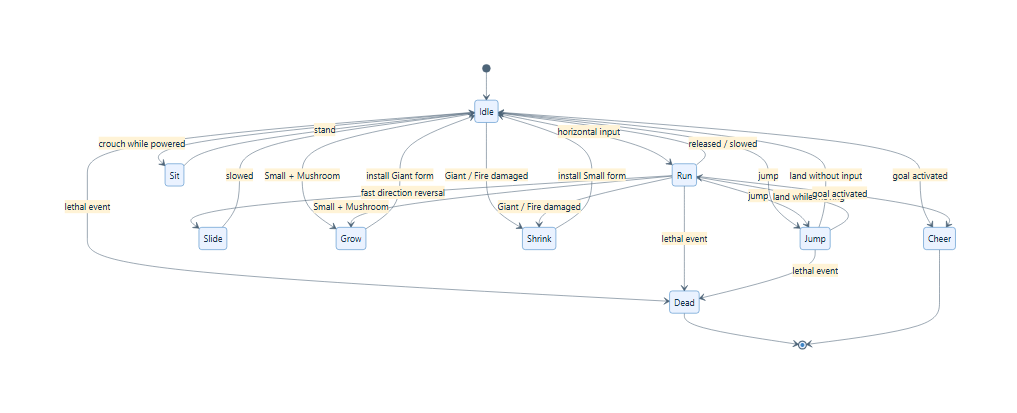
\includegraphics[width=0.98\textwidth,height=0.58\textheight,keepaspectratio]{img/diagrams/project-hero-state.png}
\caption{Principal transitions in the hero state machine.}
\label{fig:hero-state-machine}
\end{figure}

Idle, Run, Jump, Slide, and Sit own input-sensitive motion.  They use values
from \texttt{PhysicsConstants.h} for acceleration, friction, air control, jump
impulse, and fall speed.  Grow and Shrink are timed animation states.  Sit
temporarily changes a powered hero to a $32\times48$ hitbox and restores the
$32\times64$ standing hitbox on exit.  Dead owns defeat motion without terrain
collision, and Cheer locks velocity during level completion.

\subsection{Enemy and Boss System}

\subsubsection{Enemy hierarchy and composition}

\begin{figure}[htbp]
\centering
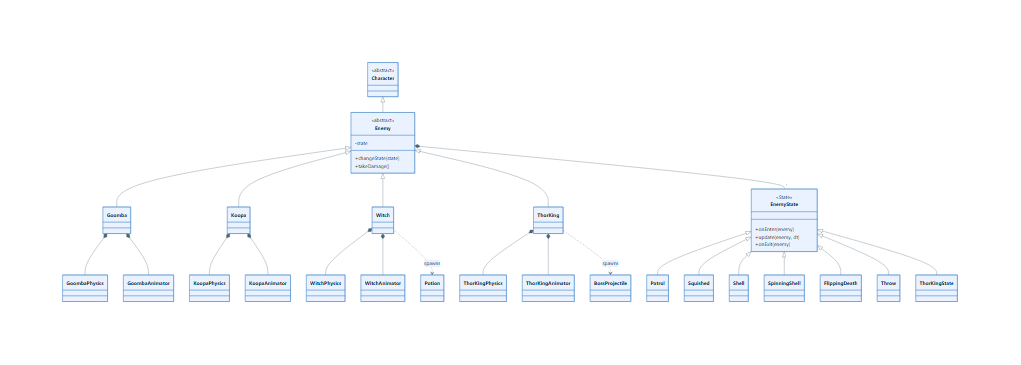
\includegraphics[width=0.99\textwidth,height=0.53\textheight,keepaspectratio]{img/diagrams/project-enemy.png}
\caption{Enemy inheritance, AI states, and composed helpers.}
\label{fig:enemy-class-diagram}
\end{figure}

\texttt{Enemy} supplies speed, health, patrol bounds, direction, sprite offset,
state timer, and the current \texttt{EnemyState}.  Patrol behavior checks bounds,
moves, and animates.  General collision responses damage the other character
or die when stomped, while subclasses refine those rules.

\texttt{Goomba} delegates movement/contact details to \texttt{GoombaPhysics}
and visual state to \texttt{GoombaAnimator}; a stomp uses a timed squished
state.  \texttt{Koopa} adds static and spinning shell modes, shell speed, wake
timer, kick cooldown, and shell-specific stomp and side-contact behavior.
Spinning shells can defeat other enemies through \texttt{InteractionSystem}.

\texttt{Witch} adds an attack cooldown and \texttt{ThrowState}.  At the attack
moment it creates an enemy-faction \texttt{Potion} through its callback.  A
potion follows gravity, becomes a wide temporary puddle on solid impact, and
can damage the hero during target interaction.

\subsubsection{Thor King boss}

\texttt{ThorKing} has three HP-based phases, increasing roll/fire behavior,
wall-bounce counters, a shot sequence, and a phase-three sky-launch cycle.
Its AI states separate patrol, crouch, rolling shell, vulnerable stun, fire
attack, and phase-change roar.  \texttt{ThorKingPhysics} owns boss collision and
damage transitions; \texttt{ThorKingAnimator} selects normal, enraged,
sky-meteor, and winged visual resources.  The boss publishes attack and defeat
sound events and can spawn straight or sky-drop attacks.  Its core HP and
counters are persisted, while transient AI resumes from a safe patrol state on
load.

This design keeps the general enemy contract usable by world systems.  The boss
is still an \texttt{Enemy}, so ordinary rendering, ownership, projectile target
selection, cleanup, and score rules apply.  Boss-specific behavior is isolated
to its class, helpers, AI states, arena code, and visual effects.

\subsection{Blocks and Items}

\subsubsection{Class diagram}

\begin{figure}[htbp]
\centering
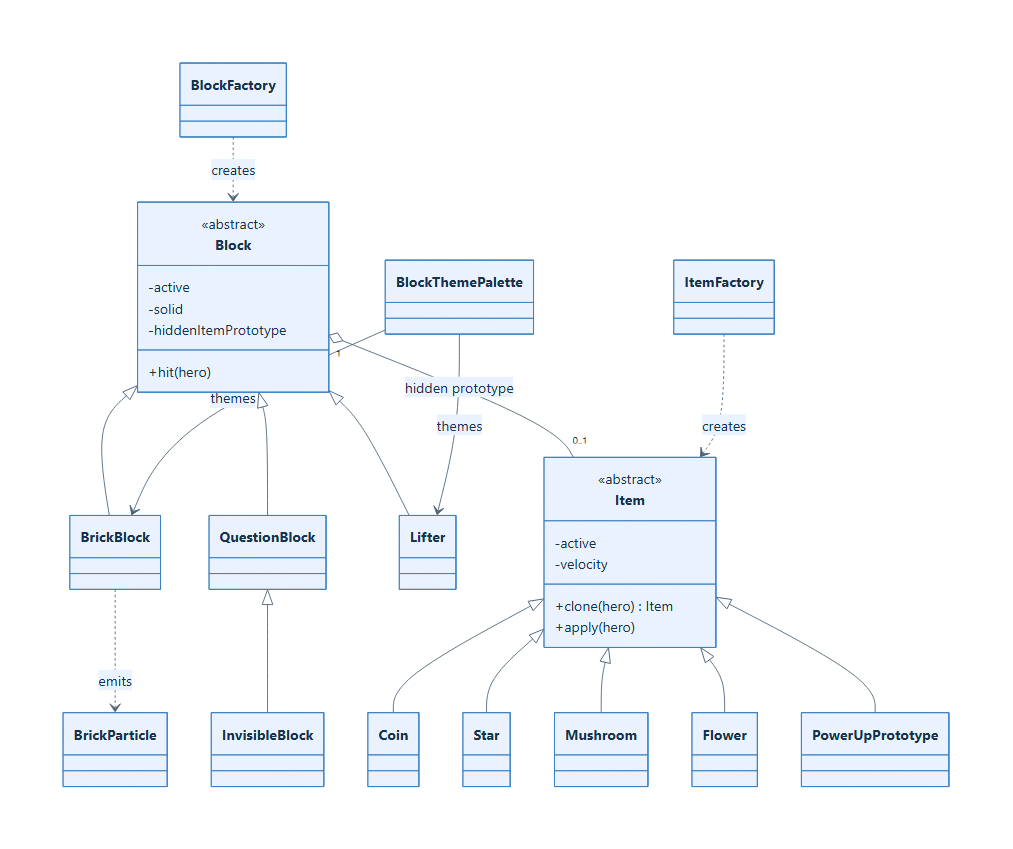
\includegraphics[width=0.97\textwidth,height=0.64\textheight,keepaspectratio]{img/diagrams/project-blocks-items.png}
\caption{Block, hidden-item Prototype, and collectible hierarchies.}
\label{fig:block-item-diagram}
\end{figure}

\texttt{Block} defines update, render, hit, lifetime, solidity, underside-hit
capability, and platform velocity.  It may own an item prototype and count.
\texttt{QuestionBlock} animates until its final hidden item is released and
then displays its empty frame.  \texttt{InvisibleBlock} derives from it but is
invisible and non-solid until hit from below.  \texttt{BrickBlock} either
releases its hidden item or, for Giant/Fire heroes, becomes four locally owned
\texttt{BrickParticle} records before deactivation.  \texttt{Lifter} is a
non-hittable solid platform that loops vertically between paired map bounds and
reports velocity so the physics system can carry a rider.

\texttt{BlockThemePalette} owns overworld, underground, and castle textures for
bricks and lifters.  The active playable-region theme selects the current
texture, so the same block objects can render correctly after pipe travel.
Blocks cache the bound theme but resynchronize during update/render.

\texttt{Item} defines spawning, cloning, collection, collision capability, and
movement data.  A ground Coin remains until collected; a block Coin is awarded
when cloned and performs a short bounce visual.  Mushroom emerges and begins
horizontal motion; Flower emerges without horizontal movement; Star emerges
and then bounces with temporary Starman invincibility on collection.
\texttt{PowerUpPrototype} chooses Mushroom or Flower at release time.  This
separation lets Tiled specify content and count while entity classes retain the
actual gameplay effects.

\subsection{Projectile System}

\begin{figure}[htbp]
\centering
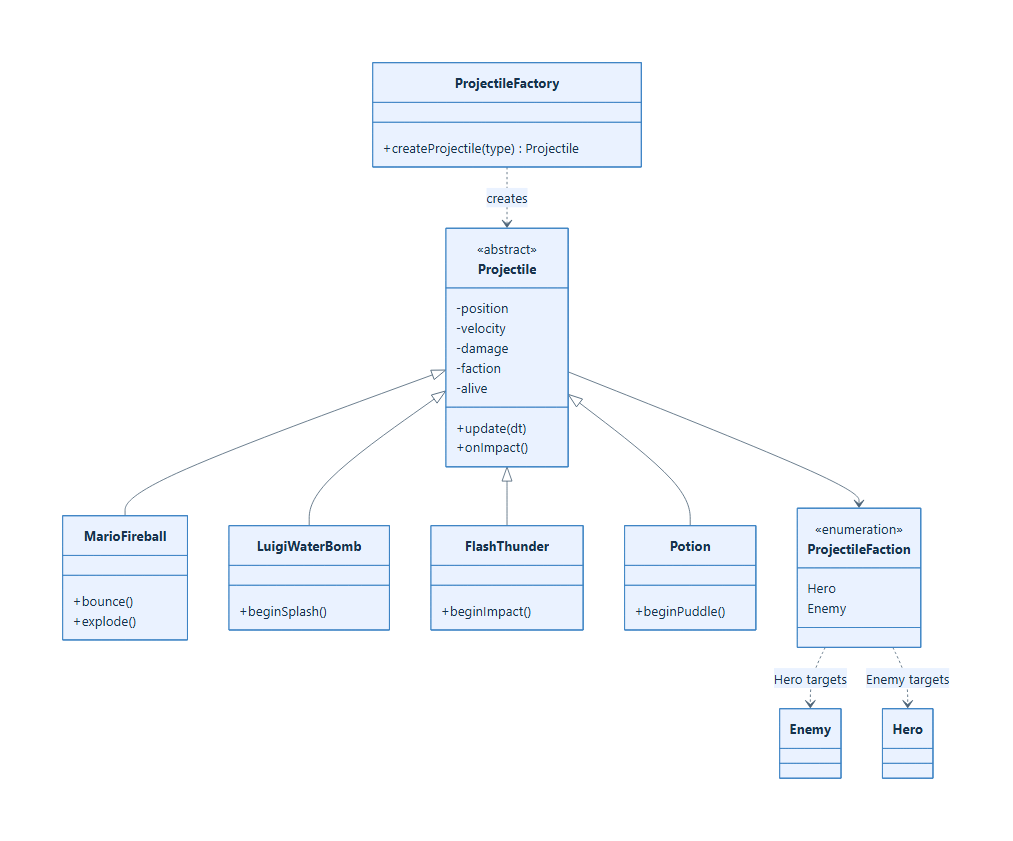
\includegraphics[width=0.92\textwidth,height=0.62\textheight,keepaspectratio]{img/diagrams/project-projectiles.png}
\caption{Unified projectile hierarchy and concrete phase behavior.}
\label{fig:projectile-class-diagram}
\end{figure}

The abstract \texttt{Projectile} contract separates intrinsic behavior from
world integration.  A projectile updates acceleration and phase timers, while
\texttt{WorldPhysicsSystem} integrates it only when
\texttt{usesWorldPhysics()} is true.  On collision, the system calls the
polymorphic \texttt{onSolidCollision}; target damage is handled through
\texttt{onHitTarget}.  \texttt{ProjectileFaction} prevents hero attacks from
targeting the hero and enemy attacks from targeting enemies.

\texttt{MarioFireball} follows gravity, bounces from floor contacts, and
explodes on walls or targets.  \texttt{LuigiWaterBomb} follows a strong arc and
expands into a one-frame damage splash.  \texttt{FlashThunder} travels without
gravity and expands into a pulsing impact strike.  Both area attacks retain a
set of already-hit character addresses and close their damage window after the
interaction pass.  \texttt{Potion} is the Witch's enemy projectile and becomes
a timed puddle.  \texttt{ProjectileFactory} reconstructs supported projectiles
from save strings while restoring velocity and faction.

\subsection{Physics and Interaction Systems}

\subsubsection{Class relationships}

\begin{figure}[htbp]
\centering
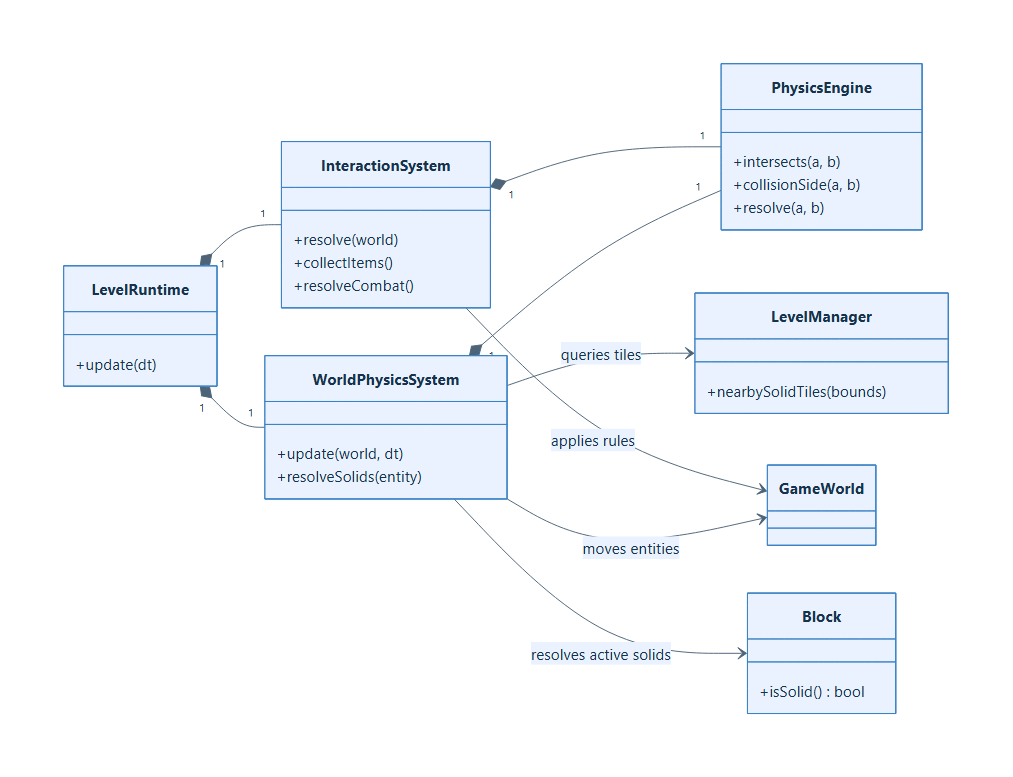
\includegraphics[width=0.96\textwidth,height=0.56\textheight,keepaspectratio]{img/diagrams/project-physics.png}
\caption{Separation between world collision and semantic interaction.}
\label{fig:physics-interaction-diagram}
\end{figure}

\texttt{PhysicsEngine} is the low-level axis-aligned bounding-box utility.  It
applies gravity, classifies a contact as Top, Bottom, Left, Right, or None, and
resolves X or Y overlap for either \texttt{sf::RectangleShape} or
\texttt{sf::FloatRect} obstacles.  \texttt{CollisionTypes.h} owns the shared
\texttt{SideType} enumeration.

\texttt{WorldPhysicsSystem} has four category-specific passes.  Hero collision
uses swept previous/proposed bounds to prevent tunneling and to select one
deterministic ceiling or landing surface.  It supports dynamic blocks, hidden
block hits, rider carry on downward lifters, grounded state, and separate X/Y
resolution.  Items integrate their velocity, land on solids, and reverse on
horizontal contacts.  Enemies receive gravity, collide with nearby terrain and
blocks, and notify or flip once on a wall.  Projectiles use their own gravity
policy and receive a polymorphic collision callback.

For performance, terrain collision enumerates only tile coordinates touched by
a swept query rectangle and asks \texttt{LevelManager::isSolidAtTile}.  It does
not scan every solid rectangle in a large level on every entity frame.  Dynamic
blocks remain a separate vector because their state, visibility, and position
can change.

\texttt{InteractionSystem} resolves semantic contacts in this order: hero-item,
spinning-shell/enemy, hero-enemy, projectile-target, and hero-goal.  It returns
one accumulated score delta.  Dead heroes and defeated/transitional enemies are
guarded consistently.  Hero area projectiles receive two target passes because
the first hit may expand their bounds; a per-frame set prevents resolving one
enemy twice.

Keeping the two systems separate is a major design decision.  A wall collision
changes geometry and velocity, while an item collection or enemy stomp changes
game semantics, score, audio, form, and lifetime.  Separating them makes the
per-frame order visible and prevents one monolithic collision routine from
knowing every concrete entity type.

\subsection{Goal and Level-Completion System}

\begin{figure}[htbp]
\centering
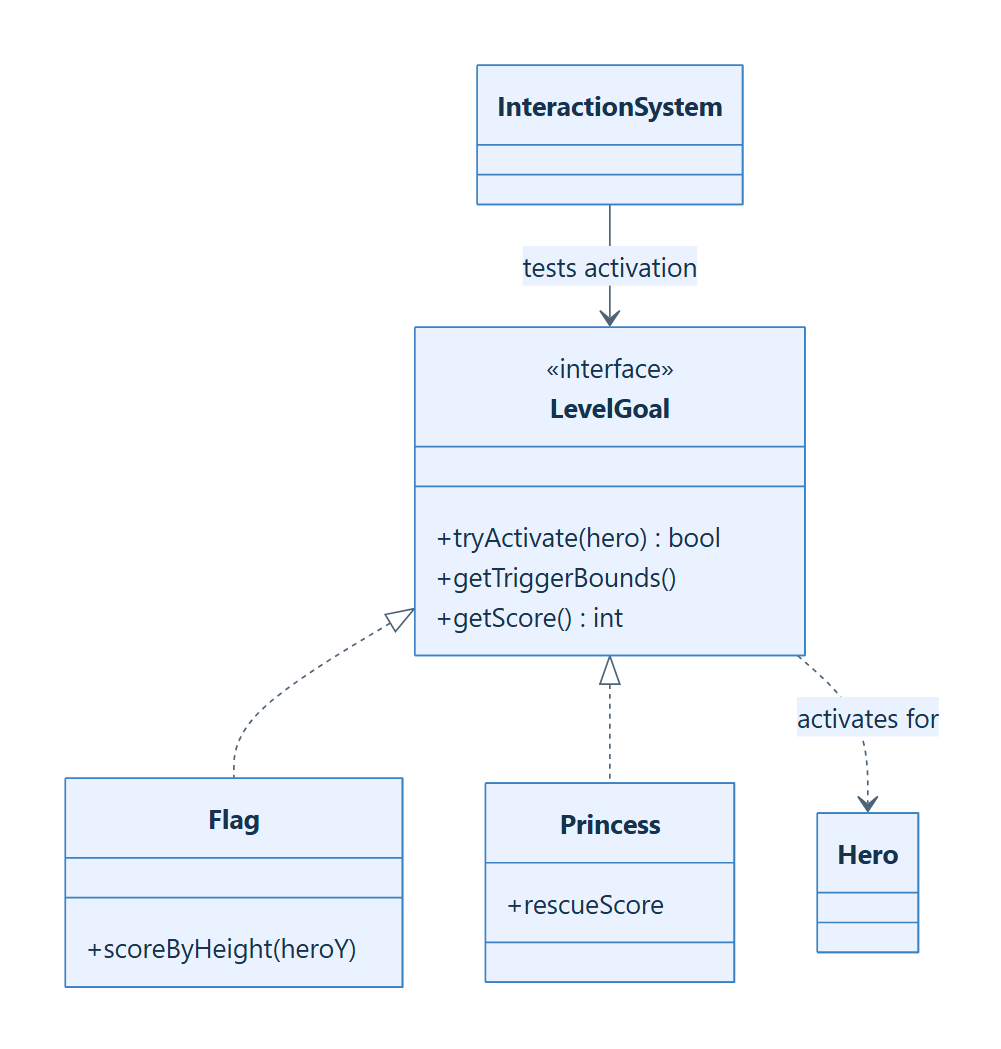
\includegraphics[width=0.66\textwidth,height=0.62\textheight,keepaspectratio]{img/diagrams/project-goals.png}
\caption{Polymorphic level goals.}
\label{fig:goal-class-diagram}
\end{figure}

\texttt{LevelGoal} is a non-rendering gameplay interface with a trigger,
activation state, score result, activation effect, and completion music.
\texttt{Flag} calculates a score between configured minimum and maximum values
from the hero's vertical contact position.  \texttt{Princess} awards a fixed
rescue score and selects its own completion cues.  The map remains responsible
for visual goal tiles; the goal object represents only semantic activation.

\texttt{InteractionSystem} attempts activation after all harmful interactions
for the frame and returns the award.  \texttt{PlayingState} observes the
activated goal, locks the hero in Cheer state, plays completion music, and opens
the Victory overlay.  This divides domain policy (whether/what a goal awards)
from screen policy (how completion is presented and where navigation goes).

\subsection{Save, Load, HUD, and Audio Services}

\subsubsection{Persistence class diagram and workflow}

\begin{figure}[htbp]
\centering
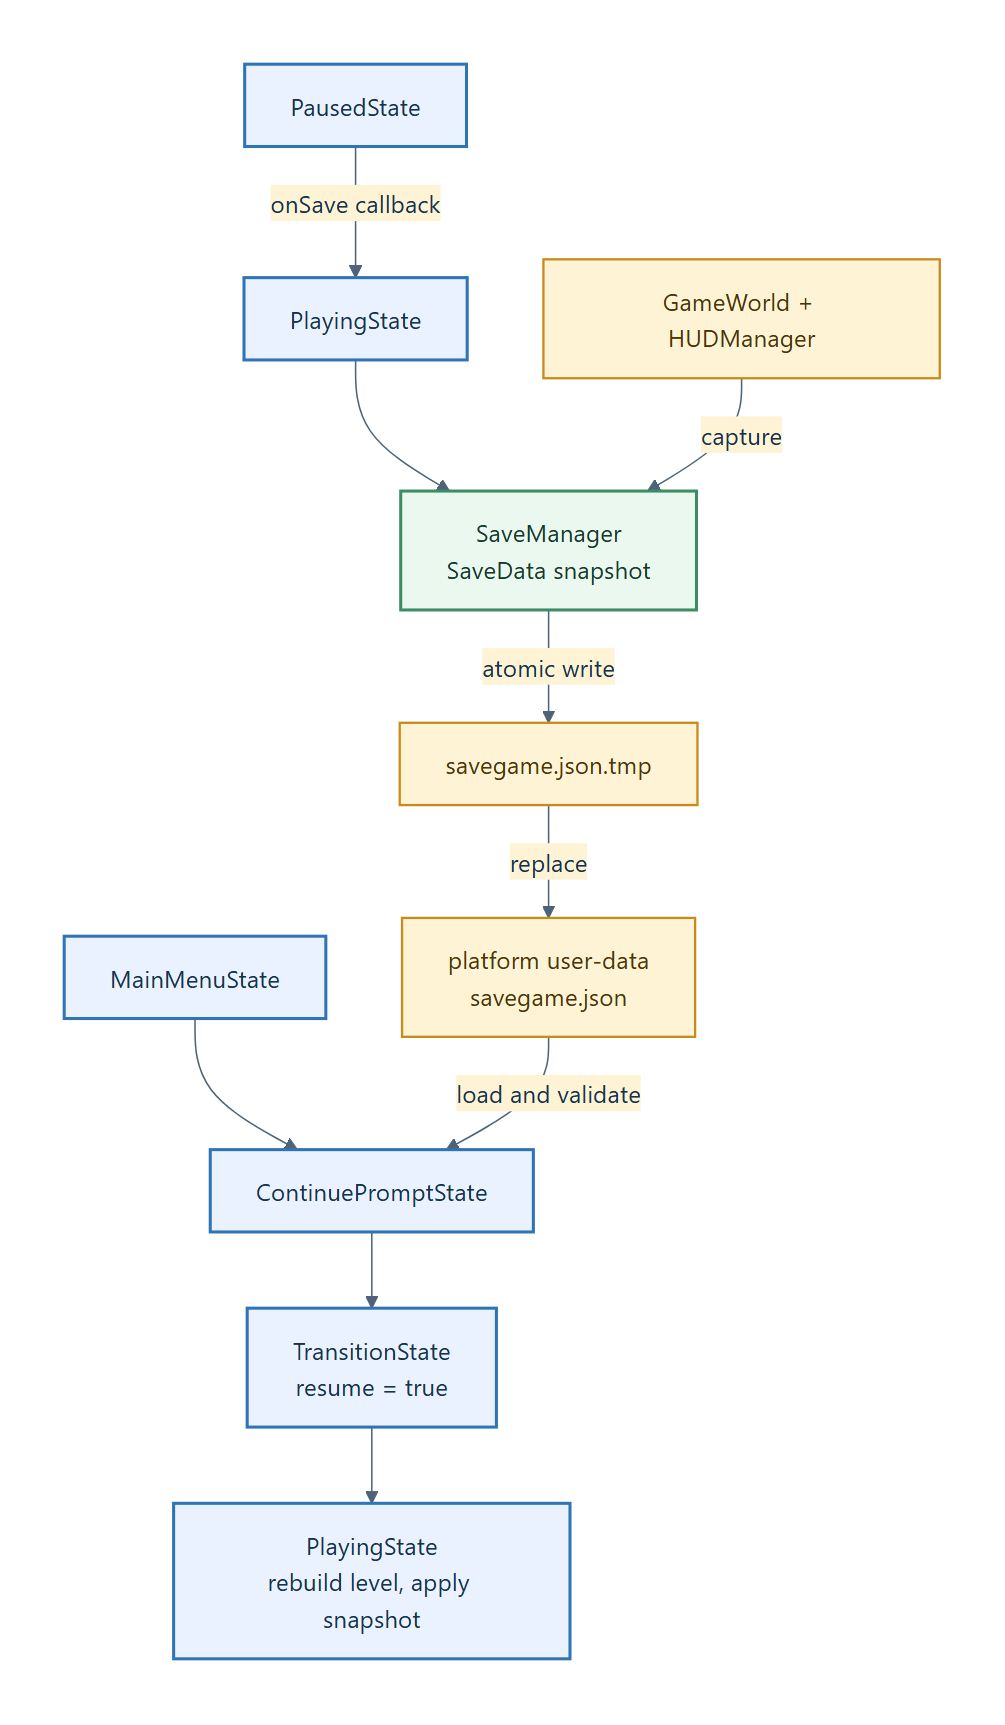
\includegraphics[width=0.66\textwidth,height=0.72\textheight,keepaspectratio]{img/diagrams/project-persistence.png}
\caption{Pause-save and menu-continue workflow.}
\label{fig:save-load-diagram}
\end{figure}

\texttt{SaveData} records map and tileset paths; hero position, HP, coins, type,
form, invincibility and Starman state; alive enemy position, velocity,
direction, health, grounded flag and AI state; additional Thor King counters;
hit and destroyed blocks; active item type and position; active projectile
type, position, velocity, and faction; and HUD score, coins, lives, and time.

\texttt{SaveManager::defaultSavePath} chooses a per-user application-data
directory on Windows, macOS, and other systems.  \texttt{existingSavePath}
also searches legacy working-directory locations.  Saving serializes JSON to a
temporary file, flushes and closes it, and then atomically replaces the target
where the operating system permits.  This is safer than truncating the only
valid save before a complete new snapshot is available.

Loading validates the JSON root, required level paths, hero object, supported
hero name, array types, and projectile faction before replacing in-memory
\texttt{SaveData}.  Continue first rebuilds the referenced level so static map
content and callbacks exist, then \texttt{applySaveToWorld} replaces the hero,
enemies, items, and projectiles through their factories, updates block/map
state, restores HUD values, and synchronizes camera region and music.

The persistence model is a snapshot, but not every transient variable is
captured.  Hero velocity, grounded/movement state, item velocity/spawn phase,
projectile lifetime/impact phase, lifter phase, activated goals, active region,
and exact boss AI timer are recomputed or reset.  This is a deliberate current
boundary: it produces a playable continuation but not bit-for-bit deterministic
resumption of the prior frame.  A future versioned save schema should add an
explicit format version and stable identifiers if exact restoration is needed.

\subsubsection{HUD}

\texttt{HUDManager} is both the model for score, coins, lives, world label, and
remaining time and an \texttt{sf::Drawable} view of those values.  Mutation
methods immediately regenerate the displayed strings.  \texttt{PlayingState}
applies score deltas from \texttt{LevelRuntime}, observes hero coin changes,
sets the compact world label from \texttt{LevelCatalog}, updates time, and
performs attempt/life restoration.  A shared pointer lets the same HUD survive
Transition, Playing, and Victory states.

\subsubsection{Audio}

\texttt{SoundManager} scans an SFX directory into named
\texttt{sf::SoundBuffer} objects, reuses a bounded pool of
\texttt{sf::Sound} channels, and streams one \texttt{sf::Music} track for BGM.
It supports independent SFX/BGM volumes and a master-volume operation.
\texttt{Game} owns it, settings modify it, screens select menu/game/result
music, and gameplay systems request effects directly or through callbacks.
Keeping the service above the level ensures music and volume survive state
replacement.

\subsection{Animation, Textures, and Other Utilities}

\begin{figure}[htbp]
\centering
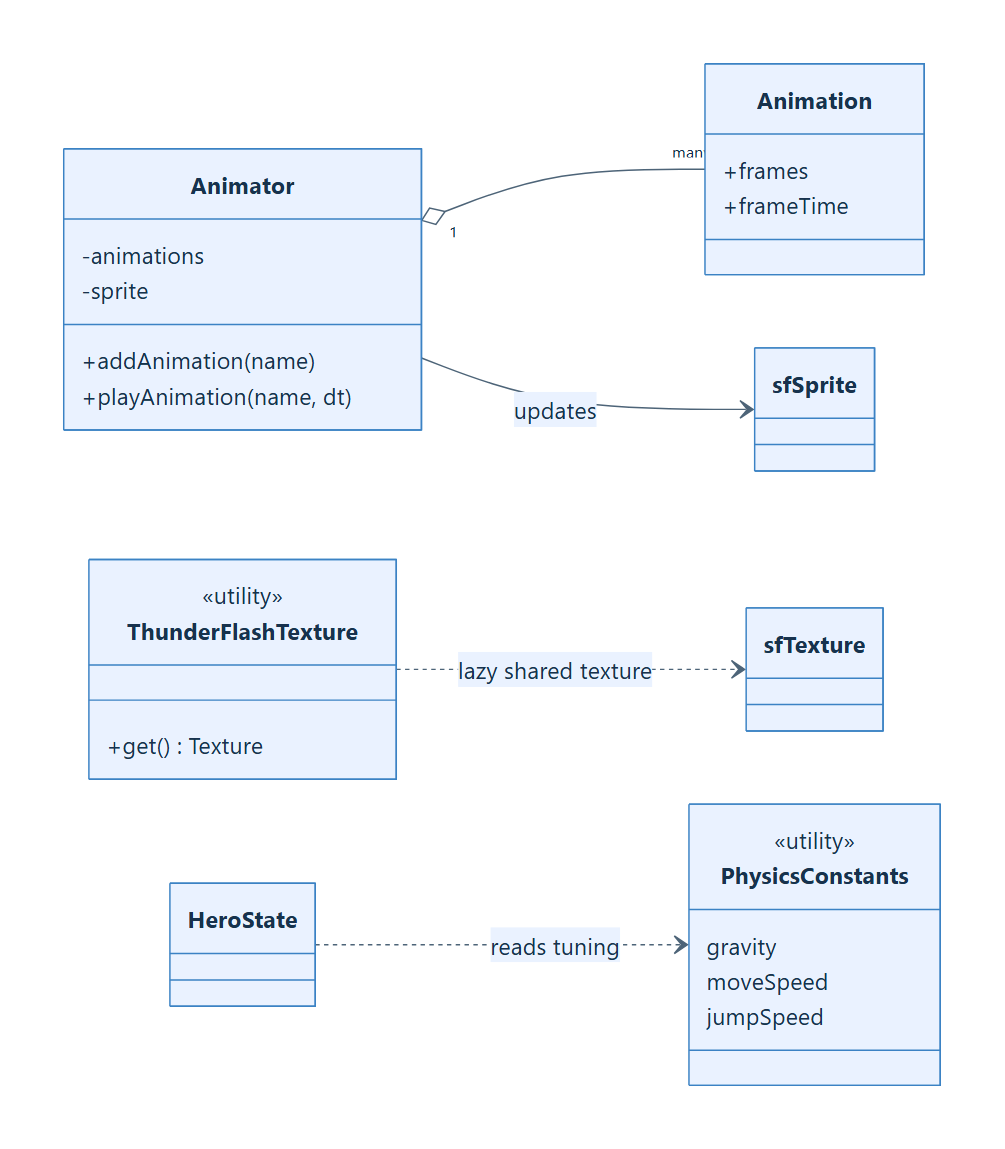
\includegraphics[width=0.88\textwidth,height=0.52\textheight,keepaspectratio]{img/diagrams/project-utilities.png}
\caption{Reusable animation and texture utilities.}
\label{fig:utility-diagram}
\end{figure}

\texttt{Animation} stores frame rectangles and duration, while
\texttt{Animator} stores named animations and mutates a referenced
\texttt{sf::Sprite}'s texture rectangle over time.  Characters, blocks, items,
and selected projectiles reuse this component.  Concrete hero constructors
register the combined form/state keys required by \texttt{Hero::update}.

\texttt{ThunderFlashTexture::get} lazily loads and transparency-processes the
Thunder Flash sheet and returns a shared non-owning texture pointer.  Lazy
creation ensures an SFML graphics context exists before the OpenGL resource is
initialized and avoids processing the same image for every Flash-related
object.  \texttt{PhysicsConstants.h} centralizes hero movement tuning rather
than scattering values across movement states.

\subsection{Ownership, Coupling, and Extension Rationale}

The principal ownership rules are:

\begin{itemize}
    \item \texttt{Game} uniquely owns screen states and the audio service;
    \item \texttt{PlayingState} owns its \texttt{LevelRuntime} by value and
    shares one HUD across related states;
    \item \texttt{LevelRuntime} owns the world and systems by value;
    \item \texttt{GameWorld} uniquely owns the hero and all entity instances;
    \item \texttt{Hero} uniquely owns its form and movement state;
    \item \texttt{Enemy} uniquely owns its AI state;
    \item \texttt{Block} uniquely owns a hidden item prototype; and
    \item pointers to \texttt{SoundManager}, references to
    \texttt{BlockThemePalette}, and callback captures are non-owning.
\end{itemize}

This arrangement avoids cycles among smart pointers.  Spawn callbacks transfer
\texttt{unique\_ptr} ownership outward to the world, while notifications carry
events without exposing the world's internals.  Abstract bases are used where
the world needs uniform lifetime/update/render behavior.  Capability methods
such as \texttt{isSolid}, \texttt{canBeHitFromBelow},
\texttt{usesWorldPhysics}, and \texttt{onSolidCollision} are preferred over
concrete casts; casts remain for explicitly boss-specific behavior.

To add a hero, implement the concrete texture/animation table and special
projectile Factory Method, add a \texttt{HeroType} and factory mapping, then add
selection UI and save parsing.  To add an enemy, implement its state/physics/
animation requirements, add an enemy factory mapping, recognize its Tiled
spawner class, and add save support if it has unique transient data.  To add a
level, add the TMJ/TSX-compatible data, a \texttt{LevelCatalog} entry, valid
start/end triggers, and only those playable regions/pipes/boss markers intended
by the design.  These extension paths explain why construction, simulation,
and presentation are separated.

\subsection{Current Constraints and Improvement Opportunities}

The current design is coherent but has several explicit trade-offs:

\begin{itemize}
    \item entity, state, form, animation, Tiled-class, and audio identifiers are
    strings in multiple boundaries; centralized constants or typed IDs would
    reduce spelling-dependent behavior;
    \item Observer behavior is callback/direct-notification based rather than a
    reusable typed event system, and coin synchronization is currently polled;
    \item some constructors load textures independently, so a general asset
    cache would reduce duplicate I/O and texture memory;
    \item state updates and most interactions use linear scans; spinning-shell
    and projectile targeting can become quadratic with many enemies, so spatial
    partitioning would be the next scaling step;
    \item the level builder still materializes a rectangle for each solid tile
    even though active collision uses nearby tile-grid queries; removing or
    repurposing the redundant collection would reduce large-level memory and
    load work;
    \item boss VFX and debug phase/form hotkeys are currently in
    \texttt{PlayingState}; a dedicated boss encounter/presentation component
    would keep the scene controller smaller;
    \item save files have validation but no schema version or migration layer;
    and
    \item there is no project-owned automated test target in the current CMake
    configuration, so regression verification depends on builds and manual play.
\end{itemize}

These are evolution points, not reasons to collapse the present subsystem
boundaries.  Improvements should preserve world ownership, deferred cleanup,
the physics/interaction split, and state-transition safety.

\subsection{Build and Deployment Structure}

\texttt{CMakeLists.txt} declares a C++17 executable named
\texttt{Custom2DPlatformer}, obtains SFML 2.6.1 through CMake FetchContent,
recursively includes project source/header directories, and links SFML graphics,
window, system, and audio libraries statically.  A post-build command copies
the complete \texttt{assets} directory beside the executable.  On Windows it
also copies the architecture-correct \texttt{openal32.dll}, because SFML's
OpenAL audio backend remains a runtime dependency even when SFML itself is
linked statically.  This explains why asset paths are relative to the executable
working directory and why both assets and OpenAL must accompany a distributed
binary.

\subsection{Complete Source-File Catalogue}
\label{subsec:source-file-catalogue}

This catalogue accounts for every current project-owned C++ header and source
file.  A notation such as \path{X.h / X.cpp} denotes the declaration and its
implementation at the corresponding \path{include} and \path{src} paths.
Interface-only headers are identified explicitly.

\begingroup
\Urlmuskip=0mu plus 1mu\relax

\subsubsection{Bootstrap and core application}

\begin{itemize}
    \item \path{src/main.cpp}: process entry point and Windows I/O
    compatibility shim.
    \item \path{include/Core/Game.h} /
    \path{src/Core/Game.cpp}: singleton application object, loop, audio,
    state stack, selection, and deferred transitions.
    \item \path{include/Core/State.h}: abstract screen-state interface.
    \item \path{include/Core/CollisionTypes.h}: shared collision-side enum.
    \item \path{include/Core/PhysicsEngine.h} /
    \path{src/Core/PhysicsEngine.cpp}: AABB collision and resolution helpers.
    \item \path{include/Core/LevelCatalog.h}: compile-time level metadata and
    next-level lookup.
\end{itemize}

\subsubsection{Screen states}

\begin{itemize}
    \item \path{include/Core/MainMenuState.h} /
    \path{src/Core/MainMenuState.cpp}.
    \item \path{include/Core/ContinuePromptState.h} /
    \path{src/Core/ContinuePromptState.cpp}.
    \item \path{include/Core/CharacterSelectState.h} /
    \path{src/Core/CharacterSelectState.cpp}.
    \item \path{include/Core/LevelSelectState.h} /
    \path{src/Core/LevelSelectState.cpp}.
    \item \path{include/Core/GuideState.h} /
    \path{src/Core/GuideState.cpp}.
    \item \path{include/Core/SettingsState.h} /
    \path{src/Core/SettingsState.cpp}.
    \item \path{include/Core/TransitionState.h} /
    \path{src/Core/TransitionState.cpp}.
    \item \path{include/Core/PlayingState.h} /
    \path{src/Core/PlayingState.cpp}.
    \item \path{include/Core/PausedState.h} /
    \path{src/Core/PausedState.cpp}.
    \item \path{include/Core/VictoryState.h} /
    \path{src/Core/VictoryState.cpp}.
    \item \path{include/Core/GameOverState.h} /
    \path{src/Core/GameOverState.cpp}.
\end{itemize}

\subsubsection{Gameplay runtime}

\begin{itemize}
    \item \path{include/Core/Gameplay/GameWorld.h} /
    \path{src/Core/Gameplay/GameWorld.cpp}: world ownership and cleanup.
    \item \path{include/Core/Gameplay/LevelRuntime.h} /
    \path{src/Core/Gameplay/LevelRuntime.cpp}: live-level facade and frame
    pipeline.
    \item \path{include/Core/Gameplay/LevelBuilder.h} /
    \path{src/Core/Gameplay/LevelBuilder.cpp}: map-to-world construction.
    \item \path{include/Core/Gameplay/WorldPhysicsSystem.h} /
    \path{src/Core/Gameplay/WorldPhysicsSystem.cpp}: movement and solid
    collision.
    \item \path{include/Core/Gameplay/InteractionSystem.h} /
    \path{src/Core/Gameplay/InteractionSystem.cpp}: semantic contacts and
    scoring.
    \item \path{include/Core/Gameplay/BlockThemePalette.h} /
    \path{src/Core/Gameplay/BlockThemePalette.cpp}: region-sensitive block
    textures.
\end{itemize}

\subsubsection{Character and hero files}

\begin{itemize}
    \item \path{include/Entities/Character/Character.h} /
    \path{src/Entities/Character/Character.cpp}: abstract character root.
    \item \path{include/Entities/Character/Hero/Hero.h} /
    \path{src/Entities/Character/Hero/Hero.cpp}: common hero behavior.
    \item \path{include/Entities/Character/Hero/HeroFactory.h} /
    \path{src/Entities/Character/Hero/HeroFactory.cpp}: hero construction.
    \item \path{include/Entities/Character/Hero/Mario.h} /
    \path{src/Entities/Character/Hero/Mario.cpp};
    \path{include/Entities/Character/Hero/Luigi.h} /
    \path{src/Entities/Character/Hero/Luigi.cpp}; and
    \path{include/Entities/Character/Hero/Flash.h} /
    \path{src/Entities/Character/Hero/Flash.cpp}: concrete heroes.
\end{itemize}

\subsubsection{Hero form and movement-state files}

\begin{itemize}
    \item \path{include/Entities/Character/Hero/HeroForm/HeroForm.h}:
    abstract form strategy.
    \item \path{include/Entities/Character/Hero/HeroForm/SmallForm.h} /
    \path{src/Entities/Character/Hero/HeroForm/SmallForm.cpp}.
    \item \path{include/Entities/Character/Hero/HeroForm/GiantForm.h} /
    \path{src/Entities/Character/Hero/HeroForm/GiantForm.cpp}.
    \item \path{include/Entities/Character/Hero/HeroForm/FireForm.h} /
    \path{src/Entities/Character/Hero/HeroForm/FireForm.cpp}.
    \item \path{include/Entities/Character/Hero/HeroState/HeroState.h}:
    abstract movement-state interface.
    \item \path{include/Entities/Character/Hero/HeroState/IdleState.h} /
    \path{src/Entities/Character/Hero/HeroState/IdleState.cpp}.
    \item \path{include/Entities/Character/Hero/HeroState/RunState.h} /
    \path{src/Entities/Character/Hero/HeroState/RunState.cpp}.
    \item \path{include/Entities/Character/Hero/HeroState/JumpState.h} /
    \path{src/Entities/Character/Hero/HeroState/JumpState.cpp}.
    \item \path{include/Entities/Character/Hero/HeroState/SlideState.h} /
    \path{src/Entities/Character/Hero/HeroState/SlideState.cpp}.
    \item \path{include/Entities/Character/Hero/HeroState/SitState.h} /
    \path{src/Entities/Character/Hero/HeroState/SitState.cpp}.
    \item \path{include/Entities/Character/Hero/HeroState/GrowState.h} /
    \path{src/Entities/Character/Hero/HeroState/GrowState.cpp}.
    \item \path{include/Entities/Character/Hero/HeroState/ShrinkState.h} /
    \path{src/Entities/Character/Hero/HeroState/ShrinkState.cpp}.
    \item \path{include/Entities/Character/Hero/HeroState/DeadState.h} /
    \path{src/Entities/Character/Hero/HeroState/DeadState.cpp}.
    \item \path{include/Entities/Character/Hero/HeroState/CheerState.h} /
    \path{src/Entities/Character/Hero/HeroState/CheerState.cpp}.
\end{itemize}

\subsubsection{Enemy and boss files}

\begin{itemize}
    \item \path{include/Entities/Character/Enemy/Enemy.h} /
    \path{src/Entities/Character/Enemy/Enemy.cpp}: common enemy entity.
    \item \path{include/Entities/Character/Enemy/EnemyFactory.h} /
    \path{src/Entities/Character/Enemy/EnemyFactory.cpp}: static and
    polymorphic enemy factories.
    \item \path{include/Entities/Character/Enemy/EnemyState.h} /
    \path{src/Entities/Character/Enemy/EnemyState.cpp}: common AI states.
    \item \path{include/Entities/Character/Enemy/EnemyStateFactory.h} /
    \path{src/Entities/Character/Enemy/EnemyStateFactory.cpp}: saved-state
    reconstruction.
    \item \path{include/Entities/Character/Enemy/Goomba.h} /
    \path{src/Entities/Character/Enemy/Goomba.cpp},
    \path{include/Entities/Character/Enemy/GoombaPhysics.h} /
    \path{src/Entities/Character/Enemy/GoombaPhysics.cpp}, and
    \path{include/Entities/Character/Enemy/GoombaAnimator.h} /
    \path{src/Entities/Character/Enemy/GoombaAnimator.cpp}.
    \item \path{include/Entities/Character/Enemy/Koopa.h} /
    \path{src/Entities/Character/Enemy/Koopa.cpp},
    \path{include/Entities/Character/Enemy/KoopaPhysics.h} /
    \path{src/Entities/Character/Enemy/KoopaPhysics.cpp}, and
    \path{include/Entities/Character/Enemy/KoopaAnimator.h} /
    \path{src/Entities/Character/Enemy/KoopaAnimator.cpp}.
    \item \path{include/Entities/Character/Enemy/Witch.h} /
    \path{src/Entities/Character/Enemy/Witch.cpp},
    \path{include/Entities/Character/Enemy/WitchPhysics.h} /
    \path{src/Entities/Character/Enemy/WitchPhysics.cpp}, and
    \path{include/Entities/Character/Enemy/WitchAnimator.h} /
    \path{src/Entities/Character/Enemy/WitchAnimator.cpp}.
    \item \path{include/Entities/Character/Enemy/ThorKing.h} /
    \path{src/Entities/Character/Enemy/ThorKing.cpp},
    \path{include/Entities/Character/Enemy/ThorKingPhysics.h} /
    \path{src/Entities/Character/Enemy/ThorKingPhysics.cpp},
    \path{include/Entities/Character/Enemy/ThorKingAnimator.h} /
    \path{src/Entities/Character/Enemy/ThorKingAnimator.cpp}, and
    \path{include/Entities/Character/Enemy/ThorKingState.h} /
    \path{src/Entities/Character/Enemy/ThorKingState.cpp}.
    \item \path{include/Entities/Character/Enemy/Projectile.h} /
    \path{src/Entities/Character/Enemy/Projectile.cpp}: shared projectile
    abstraction retained in the enemy directory for historical compatibility.
    \item \path{include/Entities/Character/Enemy/Potion.h} /
    \path{src/Entities/Character/Enemy/Potion.cpp}: Witch projectile.
\end{itemize}

\subsubsection{Block files}

\begin{itemize}
    \item \path{include/Entities/Block/Block.h} /
    \path{src/Entities/Block/Block.cpp} and
    \path{include/Entities/Block/BlockFactory.h} /
    \path{src/Entities/Block/BlockFactory.cpp}.
    \item \path{include/Entities/Block/BrickBlock.h} /
    \path{src/Entities/Block/BrickBlock.cpp} and the declaration-only
    \path{include/Entities/Block/BrickParticle.h}.
    \item \path{include/Entities/Block/QuestionBlock.h} /
    \path{src/Entities/Block/QuestionBlock.cpp}.
    \item \path{include/Entities/Block/InvisibleBlock.h} /
    \path{src/Entities/Block/InvisibleBlock.cpp}.
    \item \path{include/Entities/Block/Lifter.h} /
    \path{src/Entities/Block/Lifter.cpp}.
\end{itemize}

\subsubsection{Item files}

\begin{itemize}
    \item \path{include/Entities/Item/Item.h} /
    \path{src/Entities/Item/Item.cpp} and
    \path{include/Entities/Item/ItemFactory.h} /
    \path{src/Entities/Item/ItemFactory.cpp}.
    \item \path{include/Entities/Item/PowerUpPrototype.h} /
    \path{src/Entities/Item/PowerUpPrototype.cpp}.
    \item \path{include/Entities/Item/Coin.h} /
    \path{src/Entities/Item/Coin.cpp}.
    \item \path{include/Entities/Item/Mushroom.h} /
    \path{src/Entities/Item/Mushroom.cpp}.
    \item \path{include/Entities/Item/Flower.h} /
    \path{src/Entities/Item/Flower.cpp}.
    \item \path{include/Entities/Item/Star.h} /
    \path{src/Entities/Item/Star.cpp}.
\end{itemize}

\subsubsection{Hero projectile and goal files}

\begin{itemize}
    \item \path{include/Entities/Projectile/ProjectileFactory.h} /
    \path{src/Entities/Projectile/ProjectileFactory.cpp}.
    \item \path{include/Entities/Projectile/MarioFireball.h} /
    \path{src/Entities/Projectile/MarioFireball.cpp}.
    \item \path{include/Entities/Projectile/LuigiWaterBomb.h} /
    \path{src/Entities/Projectile/LuigiWaterBomb.cpp}.
    \item \path{include/Entities/Projectile/FlashThunder.h} /
    \path{src/Entities/Projectile/FlashThunder.cpp}.
    \item \path{include/Entities/Goal/LevelGoal.h}: goal interface.
    \item \path{include/Entities/Goal/Flag.h} /
    \path{src/Entities/Goal/Flag.cpp}.
    \item \path{include/Entities/Goal/Princess.h} /
    \path{src/Entities/Goal/Princess.cpp}.
\end{itemize}

\subsubsection{Manager and utility files}

\begin{itemize}
    \item \path{include/Managers/MapData.hpp} /
    \path{src/Managers/MapData.cpp} and
    \path{include/Managers/MapManager.hpp} /
    \path{src/Managers/MapManager.cpp}.
    \item \path{include/Managers/LevelManager.hpp} /
    \path{src/Managers/LevelManager.cpp}.
    \item \path{include/Managers/SaveManager.hpp} /
    \path{src/Managers/SaveManager.cpp}.
    \item \path{include/Managers/HUDManager.hpp} /
    \path{src/Managers/HUDManager.cpp}.
    \item \path{include/Managers/SoundManager.hpp} /
    \path{src/Managers/SoundManager.cpp}.
    \item \path{include/Utilities/Animator.h} /
    \path{src/Utilities/Animator.cpp}.
    \item \path{include/Utilities/PhysicsConstants.h}: shared movement
    constants.
    \item \path{include/Utilities/ThunderFlashTexture.h} /
    \path{src/Utilities/ThunderFlashTexture.cpp}: shared processed texture.
\end{itemize}

Finally, \path{include/nlohmann/json.hpp} and
\path{include/nlohmann/json_fwd.hpp} are vendored third-party headers rather
than project-authored domain classes.  They are nevertheless part of the build:
\path{MapManager} uses them to parse TMJ files and \path{SaveManager} uses
them to serialize and validate save snapshots.  \path{CMakeLists.txt} is the
project's build description and completes the code/build inventory.
\par
\endgroup
\par
\endgroup

\section{Applied Design Patterns}
\label{sec:applied-design-patterns}
\begingroup
\sloppy

The project uses design patterns at several different scales.  Some patterns
control the lifetime and navigation of the application, some provide extension
points for gameplay objects, and others isolate the creation of families of
entities.  Table~\ref{tab:pattern-summary} gives the principal mapping from the
pattern vocabulary to the concrete implementation.

\begin{table}[htbp]
    \centering
    \small
    \renewcommand{\arraystretch}{1.2}
    \begin{tabular}{|p{0.16\textwidth}|p{0.34\textwidth}|p{0.39\textwidth}|}
        \hline
        \textbf{Pattern} & \textbf{Principal participants} & \textbf{Purpose in the game} \\
        \hline
        Singleton & \texttt{Game} & Provides one process-wide window, state stack, audio service, and selected character/level configuration. \\
        \hline
        Factory & \texttt{HeroFactory}, \texttt{EnemyFactory}, \texttt{BlockFactory}, \texttt{ItemFactory}, \texttt{ProjectileFactory}, \texttt{EnemyStateFactory} & Converts compact types or saved/map strings into polymorphic runtime objects. \\
        \hline
        State & Application \texttt{State}; \texttt{HeroState}; \texttt{EnemyState} & Represents screens, hero movement modes, and enemy/boss AI modes without large central conditionals. \\
        \hline
        Strategy & \texttt{HeroForm} with \texttt{SmallForm}, \texttt{GiantForm}, and \texttt{FireForm} & Changes size, texture, input capabilities, special attack policy, and damage response at run time. \\
        \hline
        Observer & Sound/projectile callbacks and HUD notifications & Propagates gameplay events to the world, sound service, and display without giving entities ownership of those receivers. \\
        \hline
        Prototype & \texttt{Item::clone}, especially \texttt{PowerUpPrototype} & Lets a block retain one item description and create context-sensitive rewards when hit. \\
        \hline
        Facade & \texttt{LevelRuntime} & Presents one update/render interface over world ownership, construction, physics, interactions, regions, pipes, and goals. \\
        \hline
        Factory Method & \texttt{Hero::createSpecialProjectile} & Allows the invariant special-ability workflow to create a hero-specific projectile. \\
        \hline
        Object Pool & \texttt{SoundManager::m\_sfxPool} & Reuses a bounded number of SFML sound channels for overlapping effects. \\
        \hline
    \end{tabular}
    \caption{Design patterns identified in the current implementation.}
    \label{tab:pattern-summary}
\end{table}

\subsection{Singleton Pattern}
\label{subsec:singleton-pattern}

\subsubsection{Intent and participants}

The Singleton pattern ensures that a class has one instance and supplies a
global access point to it.  The project applies the pattern to \texttt{Game}.
Its constructor is private, its copy constructor and assignment operator are
deleted, and \texttt{Game::getInstance()} returns a function-local static
instance.  This is the ``Meyers Singleton'' form: construction occurs on first
use, and C++ guarantees thread-safe initialization of the local static object.

\begin{figure}[htbp]
\centering
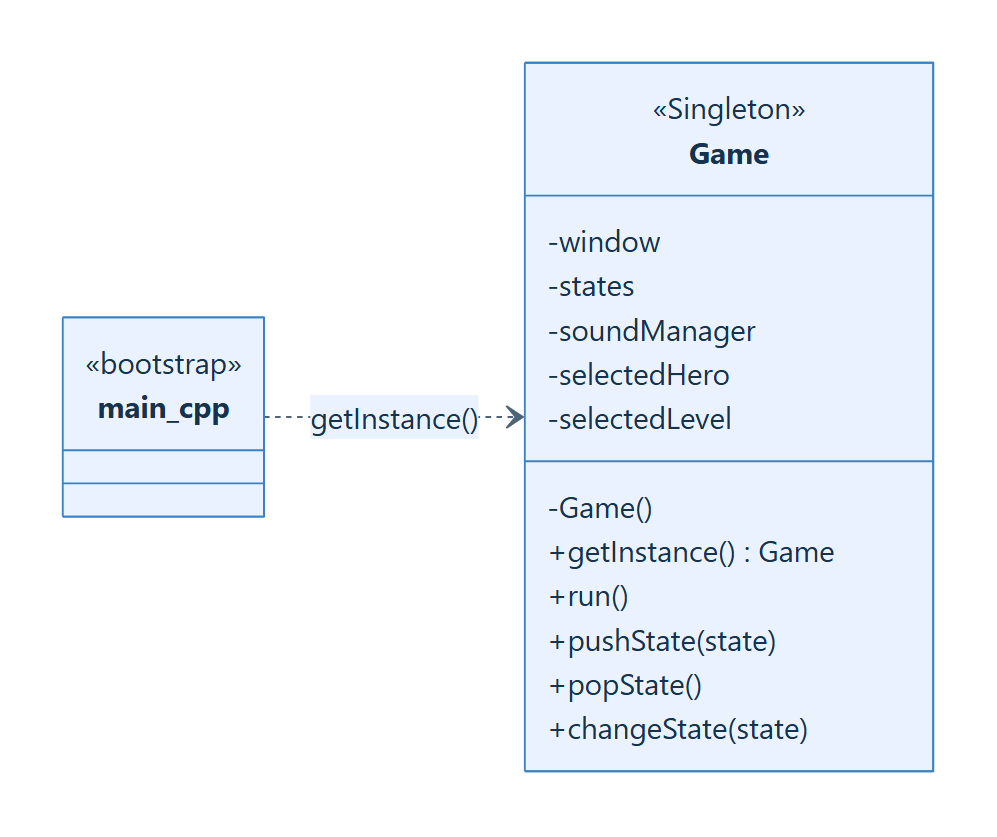
\includegraphics[width=0.56\textwidth,height=0.56\textheight,keepaspectratio]{img/diagrams/pattern-singleton.png}
\caption{The single \texttt{Game} object owns process-wide application state.}
\end{figure}

The bootstrap in \texttt{src/main.cpp} obtains the instance twice: first to
queue a \texttt{MainMenuState}, and then to start \texttt{run()}.  Screen
objects use the same access point to request state transitions, obtain the
\texttt{SoundManager}, and read or update the selected hero, selected level,
and volume settings.

\subsubsection{Why it fits}

SFML should have one authoritative render window and one main loop.  Likewise,
the state stack and deferred transition request must agree on which screen is
active.  Centralizing these resources prevents accidental creation of a second
window, independent audio service, or competing navigation stack.  The
function-local static also avoids the static-initialization-order problem that
would arise from a namespace-scope \texttt{Game} object.

The cost is global coupling: states call \texttt{Game::getInstance()} directly,
which makes isolated unit tests harder and makes dependencies less visible in
constructors.  This is acceptable for the current small application shell, but
future testing could introduce narrow interfaces such as a state navigator or
audio service and inject those interfaces while retaining a single production
\texttt{Game} instance.

\subsection{Factory Patterns}
\label{subsec:factory-patterns}

\subsubsection{Simple factories for entity families}

The project uses several centralized creation functions.  Each returns a
\texttt{std::unique\_ptr} to an abstract or base type, hiding concrete
constructors from the caller:

\begin{itemize}
    \item \texttt{HeroFactory::createHero} maps \texttt{HeroType} to
    \texttt{Mario}, \texttt{Luigi}, or \texttt{Flash}, while forwarding the
    projectile-spawn callback.
    \item \texttt{EnemyFactory::createEnemy} maps \texttt{EnemyType} to
    \texttt{Goomba}, \texttt{Koopa}, \texttt{Witch}, or \texttt{ThorKing}.
    Its string overload supports map and persistence data.
    \item \texttt{BlockFactory::createBlock} builds \texttt{BrickBlock},
    \texttt{QuestionBlock}, or \texttt{InvisibleBlock}, attaches a hidden item
    prototype, and supplies the shared \texttt{BlockThemePalette} where needed.
    \item \texttt{ItemFactory::createItem} supports both the enum-based level
    builder and the string-based save loader.
    \item \texttt{ProjectileFactory::createProjectile} reconstructs hero and
    enemy projectiles from saved type names, velocities, and factions.
    \item \texttt{EnemyStateFactory::createStateFromString} reconstructs
    ordinary enemy AI states such as \texttt{Patrol}, \texttt{Squished},
    \texttt{Shell}, \texttt{SpinningShell}, \texttt{FlippingDeath}, and
    \texttt{Throw}.
\end{itemize}

\begin{figure}[htbp]
\centering
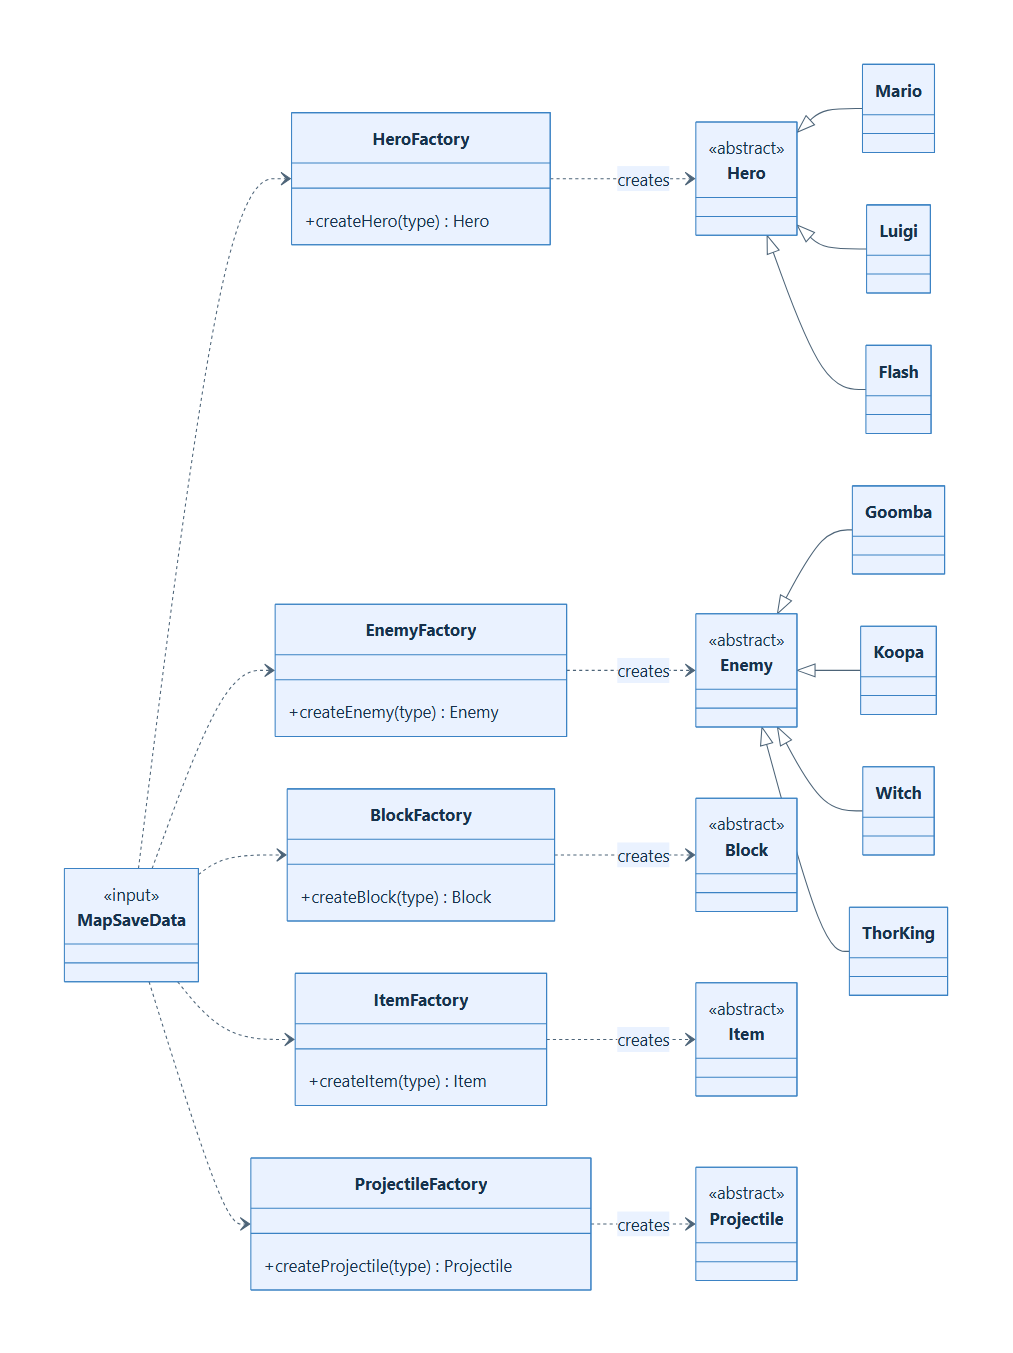
\includegraphics[width=0.68\textwidth,height=0.70\textheight,keepaspectratio]{img/diagrams/pattern-factories.png}
\caption{Factories translate data-oriented identifiers into owned polymorphic objects.}
\end{figure}

This design is especially important at the data boundary.  \texttt{LevelBuilder}
does not need sprite initialization details for every entity, and
\texttt{SaveManager} does not depend on every concrete constructor.  Adding a
new product normally requires a new concrete class, one factory mapping, and
the relevant builder or serialization mapping rather than changes throughout
the game loop.

\subsubsection{Polymorphic factory interface}

\texttt{BaseEnemyFactory} with \texttt{ConcreteGoombaFactory} and
\texttt{ConcreteKoopaFactory} is the project's explicit polymorphic factory
hierarchy.  A client can hold a \texttt{BaseEnemyFactory} reference and call
\texttt{create()} without knowing the product type.  The current runtime mainly
uses the static \texttt{EnemyFactory}; therefore the concrete factory hierarchy
is a valid extension point but is not the primary construction route.

\subsubsection{Factory Method for hero attacks}

The hero special attack is a smaller Factory Method example.  The public
\texttt{Hero::specialAbility()} method owns the stable algorithm: verify that a
spawn callback exists, ask for a projectile, and transfer ownership to the
world.  The protected pure virtual
\texttt{createSpecialProjectile()} is overridden by each hero:

\begin{itemize}
    \item \texttt{Mario} creates a bouncing \texttt{MarioFireball};
    \item \texttt{Luigi} creates an arcing \texttt{LuigiWaterBomb};
    \item \texttt{Flash} creates a fast \texttt{FlashThunder} strike.
\end{itemize}

Thus the base class fixes when and how an attack is published, while subclasses
decide what concrete product is created.

\subsection{State Pattern}
\label{subsec:state-pattern}

The project applies State three times.  These applications have the same
intent---delegating behavior to a replaceable object---but operate at different
levels and should not be confused with one another.

\subsubsection{Application and screen states}

\texttt{State} defines the common \texttt{processEvents}, \texttt{update}, and
\texttt{render} operations.  \texttt{Game} owns a stack of
\texttt{std::unique\_ptr<State>} and forwards each event/update to the top
state.  Rendering may include lower states when the top state returns
\texttt{true} from \texttt{rendersBelow()}, which is used by modal overlays such
as pause, continue prompt, and victory.

The concrete states are \texttt{MainMenuState}, \texttt{ContinuePromptState},
\texttt{CharacterSelectState}, \texttt{LevelSelectState}, \texttt{GuideState},
\texttt{SettingsState}, \texttt{TransitionState}, \texttt{PlayingState},
\texttt{PausedState}, \texttt{VictoryState}, and \texttt{GameOverState}.
Transitions are requested with \texttt{pushState}, \texttt{popState},
\texttt{changeState}, or \texttt{clearStatesAndChange}.  \texttt{Game} defers
the request until it is outside the outgoing state's callback, preventing an
object from being destroyed while one of its methods is still executing.

\begin{figure}[htbp]
\centering
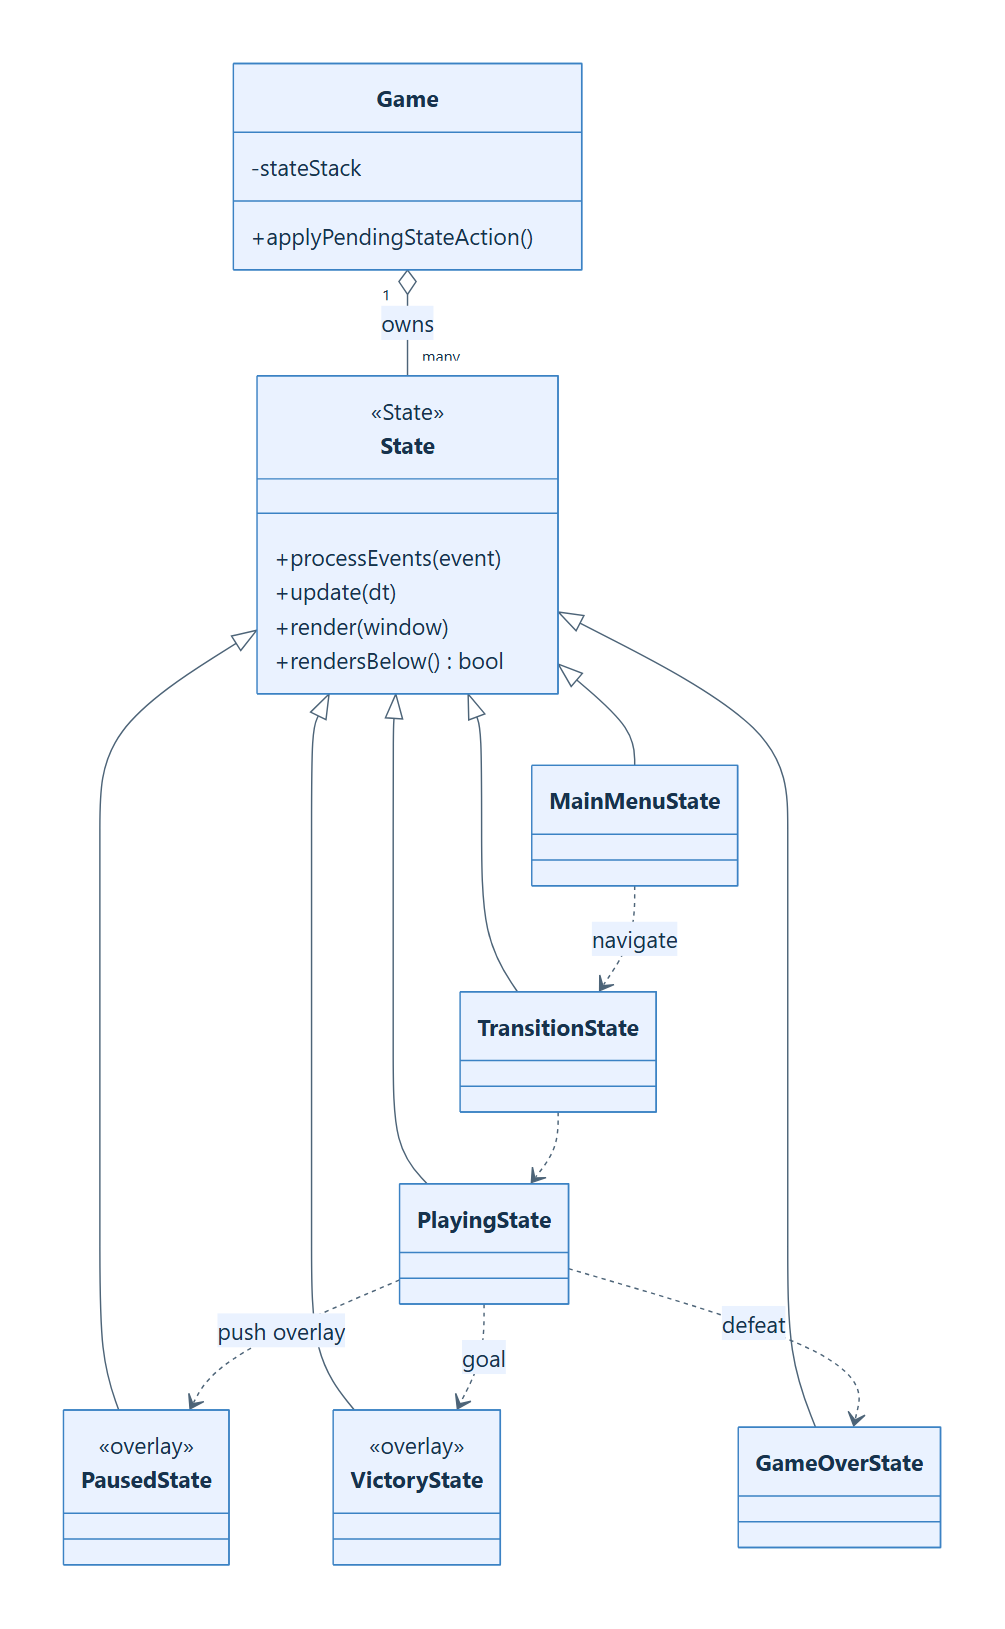
\includegraphics[width=0.68\textwidth,height=0.70\textheight,keepaspectratio]{img/diagrams/pattern-state.png}
\caption{Application State pattern and the state stack.}
\end{figure}

\subsubsection{Hero movement states}

\texttt{Hero} owns exactly one \texttt{HeroState}.  The interface supplies
\texttt{enter}, \texttt{exit}, \texttt{update}, and \texttt{getState}.  The
concrete states are \texttt{IdleState}, \texttt{RunState}, \texttt{JumpState},
\texttt{SlideState}, \texttt{SitState}, \texttt{GrowState},
\texttt{ShrinkState}, \texttt{DeadState}, and \texttt{CheerState}.  State
objects interpret input, set velocity, alter the hitbox when necessary, select
animations through their names, and initiate transitions by calling
\texttt{Hero::setState}.

For example, an idle hero enters \texttt{RunState} when horizontal input is
held, \texttt{JumpState} when jumping, and \texttt{SitState} when a powered
form crouches.  Reversing direction while moving can enter
\texttt{SlideState}.  Transformation states temporarily lock motion before
installing a new form, while \texttt{DeadState} and \texttt{CheerState} suppress
normal control for defeat and victory respectively.  \texttt{JumpState}'s
\texttt{AirEntry} value distinguishes a deliberate jump from walking off a
ledge.

\subsubsection{Enemy and boss AI states}

\texttt{Enemy} similarly owns an \texttt{EnemyState}.  Its
\texttt{changeState} method calls \texttt{onExit} on the old object and
\texttt{onEnter} on the new object.  General states implement patrolling,
squishing, a stationary shell, a spinning shell, and flipping death.
\texttt{Witch} adds \texttt{ThrowState}.  \texttt{ThorKing} extends the same
interface with \texttt{TKPatrolState}, \texttt{TKCrouchState},
\texttt{TKRollingState}, \texttt{TKStunnedState},
\texttt{TKFireAttackState}, and \texttt{TKRoarState}.  These objects express
multi-phase boss behavior while the \texttt{ThorKing} entity retains shared HP,
phase counters, movement data, projectile callback, and sound callback.

The State design localizes transition rules and makes save/load possible:
ordinary enemy state names are mapped back to state objects by
\texttt{EnemyStateFactory}.  The present persistence code restores Thor King's
counters and resumes it in a patrol state, so not every transient boss timer is
serialized.

\subsection{Strategy Pattern}
\label{subsec:strategy-pattern}

\texttt{HeroForm} is a Strategy family installed inside \texttt{Hero} alongside
the independent movement-state object.  Its operations---\texttt{enter},
\texttt{update}, \texttt{getForm}, and \texttt{takedamage}---represent the
parts of hero behavior that vary with power level rather than movement mode.

\begin{figure}[htbp]
\centering
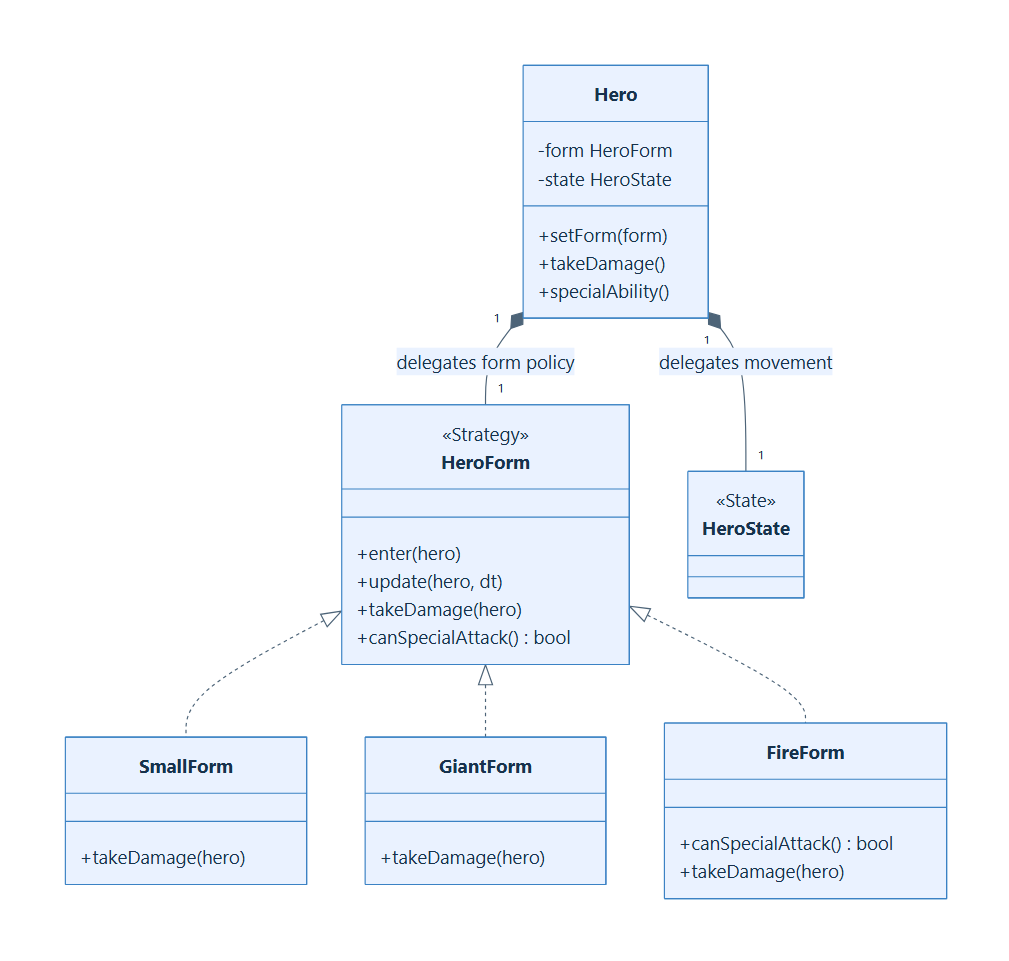
\includegraphics[width=0.82\textwidth,height=0.58\textheight,keepaspectratio]{img/diagrams/pattern-strategy.png}
\caption{Hero form is a run-time strategy independent of movement state.}
\end{figure}

\texttt{SmallForm} selects the base texture and a $32\times32$ hitbox and dies
on damage.  \texttt{GiantForm} uses a $32\times64$ standing hitbox, permits
crouching, and changes damage into a shrink transition.  \texttt{FireForm}
loads each hero's special texture, applies a per-hero cooldown, invokes the
Factory Method for the special projectile, and downgrades through Giant form
when hit.  For Mario this special strategy is Fire Mario; for Luigi it is the
Kitsune form and water bomb; for Flash it is Thunder Flash and a thunder strike.

This two-axis design prevents a combinatorial class explosion.  The project
does not require classes such as \texttt{RunningFireMario},
\texttt{JumpingGiantLuigi}, or \texttt{SittingThunderFlash}; an animation key is
instead composed from the current form and state names.  Adding a movement
state is mostly independent of adding a power form.

The enemy classes also use small statically composed policy helpers:
\texttt{GoombaPhysics}/\texttt{GoombaAnimator},
\texttt{KoopaPhysics}/\texttt{KoopaAnimator},
\texttt{WitchPhysics}/\texttt{WitchAnimator}, and
\texttt{ThorKingPhysics}/\texttt{ThorKingAnimator}.  They have no shared
strategy interface and are not swapped at run time, so they are best described
as strategy-like separation of physics and presentation rather than a complete
GoF Strategy implementation.

\subsection{Observer Pattern}
\label{subsec:observer-pattern}

The implementation uses a lightweight callback form of Observer.  It avoids
giving gameplay entities pointers to the complete scene and avoids a universal
event bus.  The significant notification channels are:

\begin{itemize}
    \item \texttt{ProjectileSpawnCallback}: \texttt{Hero} publishes a newly
    created projectile; \texttt{GameWorld::addProjectile} is the receiver.
    The same ownership-transfer idea is used by \texttt{Witch} and
    \texttt{ThorKing} for enemy projectiles.
    \item \texttt{Hero::playSFXCallback}: forms and blocks may request effects
    through the hero; \texttt{GameWorld::setHero} connects the callback to the
    non-owning \texttt{SoundManager} service.
    \item \texttt{ThorKing::m\_soundCallback}: the boss publishes
    \texttt{BossSoundEvent::Attack} and \texttt{BossSoundEvent::Defeated}; the
    level builder connects these notifications to the appropriate effects.
    \item HUD notifications: \texttt{PlayingState} observes score deltas, hero
    coin count, lives, time, and the selected world, then invokes
    \texttt{HUDManager}'s update methods.  This is explicit observation rather
    than subscription through an abstract observer interface.
\end{itemize}

\begin{figure}[htbp]
\centering
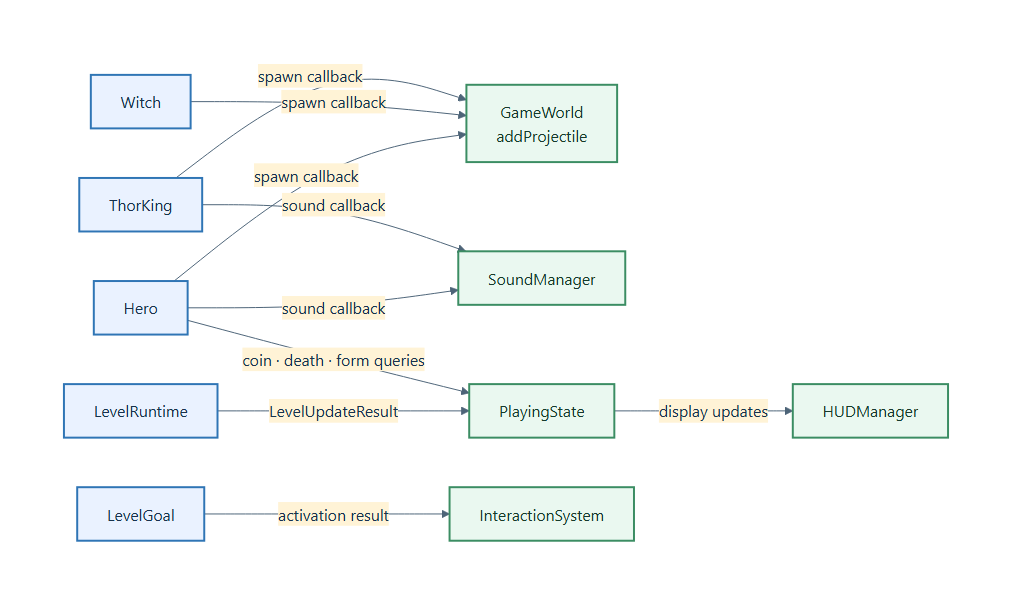
\includegraphics[width=0.94\textwidth,height=0.50\textheight,keepaspectratio]{img/diagrams/pattern-observer.png}
\caption{Callback and explicit-notification form of Observer.}
\end{figure}

The approach keeps ownership clear: a callback transfers a
\texttt{unique\_ptr} when spawning, whereas the audio pointer is non-owning and
outlives the level because it belongs to \texttt{Game}.  Its limitation is that
subscriptions are hand-wired and the HUD is partly polled, so adding many new
event consumers would justify a typed event dispatcher or formal
\texttt{Subject}/\texttt{Observer} interfaces.

\subsection{Prototype Pattern}
\label{subsec:prototype-pattern}

\texttt{Item} declares \texttt{clone(Hero*)}.  A \texttt{Block} owns one
\texttt{unique\_ptr<Item>} as its hidden prototype plus a remaining count.
When the block is hit, \texttt{releaseHiddenItem} asks the prototype to clone
itself, positions and spawns the result, decrements the count, and releases the
prototype after the last item.

The most useful prototype is \texttt{PowerUpPrototype}.  It is not itself a
visible collectible.  At clone time it examines the hero's current form and
returns a \texttt{Mushroom} for a small hero or a \texttt{Flower} for an already
powered hero.  Therefore the Tiled map can say ``power-up'' once without
hard-coding which reward is correct for the player's current context.  The
concrete \texttt{Coin}, \texttt{Star}, \texttt{Mushroom}, and \texttt{Flower}
classes also implement \texttt{clone}; coin cloning additionally awards the
coin immediately for the block-bounce visual.

\begin{figure}[htbp]
\centering
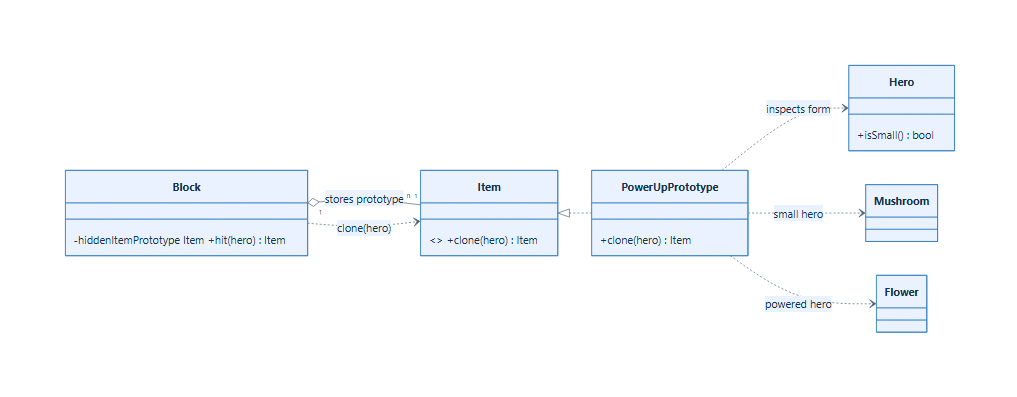
\includegraphics[width=0.88\textwidth,height=0.48\textheight,keepaspectratio]{img/diagrams/pattern-prototype.png}
\caption{Prototype supports repeated and context-sensitive hidden items.}
\end{figure}

\subsection{Facade Pattern}
\label{subsec:facade-pattern}

\texttt{LevelRuntime} is the facade for one live level.  \texttt{PlayingState}
does not directly coordinate every entity collection, collision pass, goal, or
map object.  It constructs the facade, calls \texttt{update}, calls
\texttt{renderWorld}, queries the hero and active region, and reacts to the
returned \texttt{LevelUpdateResult}.

Behind that interface, \texttt{LevelRuntime} owns \texttt{GameWorld},
\texttt{WorldPhysicsSystem}, and \texttt{InteractionSystem}; delegates initial
construction to \texttt{LevelBuilder}; caches playable regions and pipe routes;
maintains the active theme and fall boundary; enforces the boss-arena boundary;
performs cleanup; and exposes goal completion.  The facade makes the per-frame
ordering explicit while keeping scene presentation in \texttt{PlayingState}.

\subsection{Object Pool Pattern}
\label{subsec:object-pool-pattern}

\texttt{SoundManager} loads sound buffers once and keeps a bounded vector of
\texttt{sf::Sound} channels.  When an effect is requested, it first searches
for a stopped channel and reuses it; only when no stopped channel exists does it
allocate another channel, up to \texttt{m\_maxSfxChannels}.  This is a small
Object Pool that permits overlapping sound effects without allocating a new
SFML sound object for every event or allowing the number of active channels to
grow without limit.  Background music is handled separately as a streamed
\texttt{sf::Music} object.

\subsection{Pattern Collaboration and Design Consequences}
\label{subsec:pattern-collaboration}

The patterns are most valuable in combination.  The Singleton owns the screen
State context and long-lived audio service.  A selected screen constructs the
Level Facade.  The Facade delegates data-driven construction to Factories and
stores products in \texttt{GameWorld}.  During play, Hero and Enemy State
objects select short-term behavior, while the Hero Form Strategy selects the
orthogonal power policy.  Prototype creates context-sensitive block rewards,
and Observer-style callbacks publish spawned objects and sound events without
transferring control of the complete world to an entity.

The implementation consistently uses RAII ownership to reinforce these
patterns.  Screens, entities, forms, states, and projectiles are normally held
by \texttt{std::unique\_ptr}; the HUD is a \texttt{std::shared\_ptr} because it
must survive transitions and retries; service links and callback captures are
non-owning.  This makes destruction deterministic and documents whether a
relationship means ownership, sharing, or temporary collaboration.
\par
\endgroup

\section{Technical Problems and Solutions}
\label{sec:technical_problems_and_solutions}

During the development, architectural refactoring, and feature expansion of the 2D Platformer engine, several critical technical challenges emerged across the \textbf{Animation Subsystem}, \textbf{Finite State Machine (FSM)}, \textbf{Object-Oriented Hierarchy}, \textbf{World Physics Engine}, and \textbf{State Persistence Architecture}. This section details the most prominent engineering bottlenecks encountered and the mathematical, algorithmic, and architectural solutions designed to resolve them.

% =========================================================================
% SECTION 4.1
% =========================================================================
\subsection{Sprite Origin Misalignment and Center-of-Mass Jittering}
\label{subsec:sprite_misalignment}

\subsubsection{Problem Formulation}
When integrating high-resolution, non-uniform sprite sheets for advanced character forms (e.g., \textit{Epic Archmage Flash}, \textit{Fire Mario}, and \textit{Kitsune Luigi}), significant visual anomalies were observed during gameplay:
\begin{enumerate}
    \item \textbf{Horizontal Jerking / Positional Sliding:} Transitioning between discrete animation states (e.g., $\text{Idle} \rightarrow \text{Run} \rightarrow \text{Special Skill}$) caused characters to abruptly shift horizontally across the terrain.
    \item \textbf{Limb and Prop Truncation:} Attempting to eliminate jitter by tightly cropping sprite bounding boxes inadvertently severed character extremities (such as Mario's outstretched casting arm or Luigi's bushy fox tail).
\end{enumerate}

The root cause originated from the generic origin assignment implemented in the rendering utility:
\begin{equation}
    \mathbf{O}_{\text{generic}} = \left( \frac{W_{\text{rect}}}{2}, \; H_{\text{rect}} \right)
\end{equation}
Because character silhouettes within tight rectangular bounds ($W_{\text{rect}}$) are geometrically asymmetric, the bounding box midpoint $\frac{W_{\text{rect}}}{2}$ deviated substantially from the character's physical vertical anchor axis (the physical center of mass, $CM_x$), generating an instantaneous visual displacement upon every state transition.

\subsubsection{Engineering Solution}
Rather than compromising asset integrity through tight cropping or polluting the core engine with hardcoded per-frame offsets, an automated \textbf{Mathematical Center-of-Mass ($CM$) Padding Algorithm} was formulated and executed via image-processing scripts.

\paragraph{1. Center of Mass Computation:} For an arbitrary frame sub-region of width $W$ and height $H$, the horizontal center of mass is computed across all opaque body pixels:
\begin{equation}
    CM_x = \frac{\sum_{y=Y_{\min}}^{Y_{\max}} \sum_{x=X_{\min}}^{X_{\max}} x \cdot \mathbb{I}(\alpha(x, y) > \tau)}{\sum_{y=Y_{\min}}^{Y_{\max}} \sum_{x=X_{\min}}^{X_{\max}} \mathbb{I}(\alpha(x, y) > \tau)}
\end{equation}
where $\alpha(x, y) \in [0, 255]$ represents the pixel alpha channel, $\tau = 25$ is the opacity threshold, and $\mathbb{I}(\cdot)$ is the indicator function.

\paragraph{2. Symmetric Geometric Padding:} Given the calculated anchor $CM_x$ and the true visual bounds $[X_{\min}, X_{\max}]$, symmetric transparent space is injected to force the geometric midpoint to coincide with $CM_x$:
\begin{equation}
    X_{\text{rect}}, W_{\text{rect}} = 
    \begin{cases} 
        \left( X_{\min}, \; 2 \cdot (CM_x - X_{\min}) \right) & \text{if } CM_x \ge \frac{X_{\min} + X_{\max}}{2} \\
        \left( 2 \cdot CM_x - X_{\max}, \; 2 \cdot (X_{\max} - CM_x) \right) & \text{if } CM_x < \frac{X_{\min} + X_{\max}}{2}
    \end{cases}
\end{equation}
This formulation guarantees that the origin $\frac{W_{\text{rect}}}{2}$ remains strictly aligned with the character's physical foot position ($100\%$ jitter elimination) while preserving all extended visual effects and staff/tail animations.

% =========================================================================
% SECTION 4.2
% =========================================================================
\subsection{Finite State Machine (FSM) Oscillation and Frame Freezing}
\label{subsec:fsm_oscillation}

\subsubsection{Problem Formulation}
During locomotion testing, characters exhibited a severe defect where holding the movement keys caused the sprite to freeze on a single static frame while translating across the floor (appearing to ``skate'' without playing the stride animation).

Code inspection of the locomotion state machine (\texttt{RunState.cpp}) revealed an unguarded velocity threshold check:
\begin{equation}
    \text{if } (|v_x| < v_{\text{stop}}) \implies \text{Transition to } \mathtt{IdleState}
\end{equation}
When accelerating from rest, initial horizontal velocity $v_x$ initiates at $0.0\,\text{px/s}$, which is strictly below $v_{\text{stop}} = 8.0\,\text{px/s}$. Consequently, on every frame:
\begin{enumerate}
    \item \texttt{IdleState} detected keypress $\rightarrow$ transitioned to \texttt{RunState}.
    \item On the immediate subsequent tick, \texttt{RunState} detected $|v_x| < 8.0\,\text{px/s}$ $\rightarrow$ prematurely reverted to \texttt{IdleState}.
    \item This high-frequency state oscillation continuously triggered \texttt{Hero::setState()}, resetting the animation accumulator ($\mathtt{currentFrameIndex} = 0$), permanently locking the character on Frame 0.
\end{enumerate}

\subsubsection{Engineering Solution}
The transition guard was redesigned to decouple player intentionality from instantaneous kinematic magnitude by constructing a composite boolean invariant:
\begin{equation}
    \text{Transition}(\mathtt{RunState} \rightarrow \mathtt{IdleState}) \iff \left( \neg \mathtt{pressLeft} \land \neg \mathtt{pressRight} \right) \land \left( |v_x| < v_{\text{stop}} \right)
\end{equation}
This condition ensures that as long as directional input remains active, the FSM remains locked in \texttt{RunState}, allowing uninterrupted animation frame delta accumulation and fluid multi-frame locomotion.

% =========================================================================
% SECTION 4.3
% =========================================================================
\subsection{Elimination of Hardcoded Ground Constraints via Dynamic Gravity Kinematics}
\label{subsec:dynamic_gravity}

\subsubsection{Problem Formulation}
In early engine iterations, physical entities (including power-up items such as \textit{Mushrooms} and \textit{Flowers}, dynamic throwables such as \textit{Potions}, and spawned \textit{Enemies}) relied on static, hardcoded vertical offsets ($Y$-coordinates) mapped to flat ground planes. This introduced severe structural fragility:
\begin{itemize}
    \item When deploying multi-tier levels (such as underground rooms, floating platforms, and elevated pipe structures in World 1-1 and World 1-3), entities spawned with fixed parameters either hovered in mid-air or intersected solid terrain blocks.
    \item Kinematic item trajectories (e.g., mushrooms popping out of Question Blocks) lacked realistic arc landing mechanics across irregular terrain contours.
\end{itemize}

\subsubsection{Engineering Solution}
To enforce map-agnostic behavior, static spatial assumptions were eliminated in favor of a \textbf{Unified Dynamic Gravity and AABB Collision Resolution Subsystem} within \texttt{WorldPhysicsSystem}:

\paragraph{1. Kinematic Velocity Integration:} Every dynamic entity updates vertical velocity under constant gravitational acceleration:
\begin{align}
    v_y(t + \Delta t) &= \min\left(v_y(t) + g \cdot \Delta t, \; v_{\text{terminal}}\right) \\
    y(t + \Delta t) &= y(t) + v_y(t + \Delta t) \cdot \Delta t
\end{align}
where $g = 1568\,\text{px/s}^2$ and $v_{\text{terminal}} = 960\,\text{px/s}$ prevents collision tunneling through thin tile boundaries.

\paragraph{2. Continuous Ground Snapping:} During vertical collision passes against the terrain grid, ground contact is resolved dynamically:
\begin{equation}
    \text{if } \text{CollisionSide} == \mathtt{Top} \implies 
    \begin{cases}
        y_{\text{resolved}} = y_{\text{tile\_top}} - H_{\text{hitbox}} \\
        v_y = 0 \\
        \mathtt{isGrounded} = \text{true}
    \end{cases}
\end{equation}
This mathematical resolution guarantees that all characters, dropped items, and projectiles dynamically conform to arbitrary terrain topography with zero manual configuration.

% =========================================================================
% SECTION 4.4
% =========================================================================
\subsection{Polymorphic Multi-Tier Hero Evolution and Texture Routing}
\label{subsec:polymorphic_evolution}

\subsubsection{Problem Formulation}
Procedural texture loading in \texttt{HeroForm} subclasses previously invoked \texttt{hero->loadTexture(baseTexturePath)} directly upon entry. When integrating heroes with independent asset sets (e.g., \textit{Flash} utilizing \texttt{thunderflash2.png} or \textit{Luigi} utilizing \texttt{KitsuneLuigi.png}), procedural transitions caused texture coordinate mismatches and skipped growth forms, violating the \textbf{Open/Closed Principle (OCP)}.

\subsubsection{Engineering Solution}
The evolution subsystem was refactored using the \textbf{State/Strategy Pattern}:
\begin{enumerate}
    \item \textbf{Polymorphic Texture Dispatch:} Overrode \texttt{Hero::loadTexture()} in specialized classes to dynamically resolve resource bindings based on active form state.
    \item \textbf{Decoupled Multi-Tier Scaling:} Implemented independent rendering scale metrics:
    \begin{equation}
        S_{\text{render}} = 
        \begin{cases} 
            S_{\text{small}} & \text{if } \mathtt{Form} == \text{Small} \quad (32\times 32\,\text{px hitbox}) \\
            S_{\text{giant}} & \text{if } \mathtt{Form} == \text{Giant} \quad (32\times 64\,\text{px hitbox}) \\
            S_{\text{special}} & \text{if } \mathtt{Form} == \text{Fire/Special} \quad (32\times 64\,\text{px hitbox})
        \end{cases}
    \end{equation}
    \item \textbf{Uniform 3-Tier Hierarchy:} Standardized progression across all playable heroes: $\text{Small Form} \xrightarrow{\text{Mushroom}} \text{Giant Form} \xrightarrow{\text{Flower}} \text{Tier-3 Special Form}$.
\end{enumerate}

% =========================================================================
% SECTION 4.5
% =========================================================================
\subsection{World State Serialization and Dynamic Deserialization (Save/Load)}
\label{subsec:save_load_architecture}

\subsubsection{Problem Formulation}
Implementing persistent world serialization (\texttt{F5} Quick Save, \texttt{F9} Quick Load) required capturing a heterogeneous runtime state containing:
\begin{itemize}
    \item Dynamic entities (enemies with remaining state timers, active projectiles, roaming items).
    \item Spatial world modifications (permanently hit question blocks, shattered brick blocks removed from the collision matrix).
    \item Player inventory, form type, invincibility I-frames, and HUD progress metrics.
\end{itemize}

\subsubsection{Engineering Solution}
A \textbf{Base Level Reload $\rightarrow$ State Overlay Pipeline} was engineered within \texttt{SaveManager} using JSON serialization:
\begin{enumerate}
    \item \textbf{Phase 1: Deterministic Base Reload:} \texttt{LevelRuntime::reload()} re-instantiates the raw TMX/TMJ tile matrix and baseline colliders.
    \item \textbf{Phase 2: Dynamic State Overlay:}
    \begin{itemize}
        \item \textbf{Tile Matrix Mutation:} Querying coordinates $(T_x, T_y)$ against serialized \texttt{destroyedBlocks} updates the interactive vertex mesh via \texttt{setTileID("Interactive", tx, ty, 0)}.
        \item \textbf{Polymorphic Entity Reconstruction:} \texttt{EnemyFactory} and \texttt{EnemyStateFactory} reconstruct surviving enemies with precise velocity vectors and remaining AI timers (e.g., maintaining a Koopa shell's retreat countdown).
        \item \textbf{Hero State Restoration:} Re-injects exact health, coin count, form name, and remaining invulnerability duration.
    \end{itemize}
\end{enumerate}

\subsection{Dynamic Spatial Partitioning via Playable Regions and Context-Aware Theming}
\label{subsec:playable_regions}
\subsubsection{Problem Formulation}
In traditional monolithic 2D platformers, levels often encompass multiple distinct sub-environments within a single continuous tilemap (e.g., the sunny Overworld surface alongside subterranean coin chambers or deep castle arenas). Managing such multi-room levels through a single global coordinate system created three critical architectural bottlenecks:
\begin{enumerate}
    \item \textbf{Camera Viewport Bleeding:} A naive player-following camera easily drifted out of room boundaries, exposing unrendered void areas, black borders, or adjacent hidden rooms on the screen.
    \item \textbf{Static Pit-Death Invalidation:} In early iterations, the ``pit-fall'' death boundary was defined as a single hardcoded global horizontal line ($Y_{\text{death}} = Y_{\text{global\_bottom}}$). When a player entered an elevated room or a deep underground chamber situated far below the main level surface, this static threshold caused either \textit{instantaneous false deaths upon entering lower rooms} or \textit{unbounded falling through infinite space} without triggering character death.
    \item \textbf{Heterogeneous Environmental Theming:} Objects, terrain tiles, and background visual styles (e.g., vibrant Overworld vs. dark blue Underground vs. molten Castle) required dynamic context-aware rendering based strictly on the player's active containment zone.
\end{enumerate}
\subsubsection{Engineering Solution}
To resolve these spatial and visual conflicts, the engine implemented a **Data-Driven Dynamic Spatial Partitioning Architecture** based on decoupled \texttt{PlayableRegion} bounding zones and active \texttt{Theme} identifiers parsed dynamically from Tiled map triggers:
\paragraph{1. Spatial Zone Partitioning:} Each distinct chamber within the map is encapsulated by a geometric bounding volume:
\begin{equation}
    \mathcal{R}_k = \left\{ (x, y) \in \mathbb{R}^2 \;\middle|\; X_k^{\min} \le x \le X_k^{\max}, \; Y_k^{\min} \le y \le Y_k^{\max} \right\}
\end{equation}
The engine tracks the hero's position $\mathbf{P}_{\text{hero}}(t)$ and dynamically resolves the active region:
\begin{equation}
    \mathcal{R}_{\text{active}}(t) = \left\{ \mathcal{R}_k \;\middle|\; \mathbf{P}_{\text{hero}}(t) \in \mathcal{R}_k \right\}
\end{equation}
\paragraph{2. Constrained Camera Viewport Clamping:} The game camera dynamically clamps its center $(C_x, C_y)$ to ensure that the rendering viewport of dimension $(W_{\text{cam}}, H_{\text{cam}})$ never exposes out-of-bounds void:
\begin{align}
    C_x &= \text{clamp}\left( P_{\text{hero}, x}, \; X_k^{\min} + \frac{W_{\text{cam}}}{2}, \; X_k^{\max} - \frac{W_{\text{cam}}}{2} \right) \\
    C_y &= \text{clamp}\left( P_{\text{hero}, y}, \; Y_k^{\min} + \frac{H_{\text{cam}}}{2}, \; Y_k^{\max} - \frac{H_{\text{cam}}}{2} \right)
\end{align}
\paragraph{3. Dynamic Context-Aware Kill Planes:} Rather than relying on a static coordinate, the lethal pit threshold ($Y_{\text{kill}}$) for both the Hero and Enemies is computed dynamically relative to the active region's bottom boundary:
\begin{equation}
    Y_{\text{kill}}(\mathcal{R}_k) = Y_k^{\max} + \delta_{\text{threshold}}
\end{equation}
where $\delta_{\text{threshold}}$ represents the vertical grace offset before triggering \texttt{Hero::die()} or enemy entity deallocation. When traveling through pipes into an underground cavern, $Y_{\text{kill}}$ instantly re-binds to the subterranean floor baseline.
\paragraph{4. Context-Driven Visual and Audio Theming:} Each $\mathcal{R}_k$ is mapped to a dedicated environmental descriptor (\texttt{Theme::Overworld}, \texttt{Theme::Underground}, \texttt{Theme::Castle}):
\begin{equation}
    \mathcal{T}_{\text{render}} = f(\mathcal{R}_{\text{active}}) \implies 
    \begin{cases}
        \text{Background Asset \& Clear Color Binding} \\
        \text{Interactive Object / Palette Shader Dispatch} \\
        \text{Background Music (BGM) Stream Switching}
    \end{cases}
\end{equation}
\subsubsection{Resulting Impact}
This architecture completely eliminates camera visual bleeding across room transitions, guarantees mathematical accuracy for pit-fall death detection across arbitrary multi-tier map layouts, and enables rich, heterogeneous environmental theming within a single seamless level file.   
\section{Potential Future Development}

This section presents two core future expansion directions aimed at improving extensibility, personalizing the user experience, and supporting user-generated content.

\vspace{0.5cm}

\subsection{Future Direction 1: In-Game Custom Map Builder}

\subsubsection{Functional Overview}
This feature allows players to directly design 2D maps within the game interface:
\begin{itemize}
    \item Placement and removal of terrain blocks, functional blocks (\texttt{QuestionBlock}, \texttt{BrickBlock}, \texttt{Lifter}), items, enemy spawn locations (\texttt{Goomba}, \texttt{Koopa}, \texttt{Witch}, \texttt{ThorKing}), player spawn points, and destinations (\texttt{Flag}, \texttt{Princess}).
    \item Support for undo/redo operations, visual theme selection (Overworld, Underground, Castle), JSON map saving/exporting, and an instant playtest mode.
\end{itemize}

\subsubsection{Evaluation of the Current Design (OOP/SOLID Perspective)}
\textbf{Strengths (Reusability):}
\begin{itemize}
    \item The \texttt{MapData} data structure cleanly separates the tile grid layer (\texttt{TileLayer}) from the entity list (\texttt{ObjectLayer}), making it suitable as an in-memory map representation.
    \item The \texttt{LevelManager} already provides validation and update operations through \texttt{setTileID()}, along with a \texttt{VertexArray}-based batch rendering mechanism.
    \item The \texttt{LevelBuilder} and existing factories (\texttt{HeroFactory}, \texttt{BlockFactory}, \texttt{EnemyFactory}) can be reused to build a \texttt{GameWorld} from \texttt{MapData}, providing a foundation for the playtest feature.
\end{itemize}

\vspace{0.3cm}
\noindent\textbf{Weaknesses and Design Challenges (OOP/SOLID):}
\begin{itemize}
    \item \textbf{Potential Single Responsibility Principle (SRP) Violation:} If a single \texttt{MapEditorState} class is implemented to handle mouse input, UI palettes, tile-map modification, JSON serialization, and history management, it could accumulate too many responsibilities and become a God Object.
    
    \item \textbf{Limited Extensibility of Entity Registration:} Currently, entity classification in the \texttt{LevelBuilder} relies on string comparisons (e.g., \texttt{className == "goomba"}). Applying the same approach to the editor toolbar would require modifying the editor source code whenever a new entity type is introduced, limiting compliance with the Open-Closed Principle (OCP).
    
    \item \textbf{Missing Serialization Support:} The \texttt{MapManager} currently provides map loading through \texttt{loadMap()}, but does not support serializing modified map data back into the expected JSON/Tiled Map format.
\end{itemize}

\subsubsection{Proposed Architecture}
\begin{itemize}
    \item \textbf{Command Pattern (\texttt{IEditorCommand}):} Encapsulates each editing operation (e.g., placing/removing a tile, adding/removing an enemy) into command objects supporting \texttt{execute()} and \texttt{undo()}, enabling safe Undo/Redo functionality while keeping history management separate from the editor state.
    
    \item \textbf{Strategy Pattern (\texttt{IEditorTool}):} Separates editor interaction modes (\texttt{TileBrushTool}, \texttt{EraserTool}, \texttt{EntityTool}) into independent and interchangeable tool strategies.
    
    \item \textbf{Dedicated \texttt{MapSerializer}:} Separates map validation and serialization responsibilities by validating \texttt{MapData} through operations such as \texttt{validateMap()} and converting it into the required JSON format.
\end{itemize}

\begin{figure}[h]
\centering
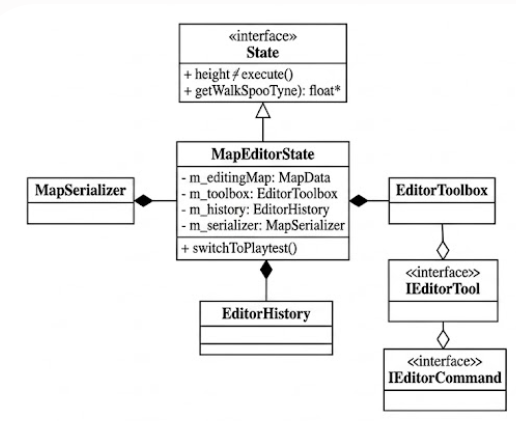
\includegraphics[width=0.45\textwidth]{img/future_suggestion_1.png}
\caption{Proposed Architecture for In-Game Map Builder}
\end{figure}

\FloatBarrier

\subsection{Future Direction 2: Data-Driven Gameplay Configuration}

\subsubsection{Functional Overview}
This feature allows players or developers to directly customize runtime gameplay parameters:
\begin{itemize}
    \item \textbf{Hero Parameters:} Walking speed, jump force, acceleration, invincibility duration, special-skill cooldown, and initial life count.
    \item \textbf{Enemy Parameters:} Maximum health, patrol speed, movement range, and attack frequency for bosses and witches.
    \item \textbf{World Physics Parameters:} Global gravity, friction coefficients, and maximum fall speed.
    \item \textbf{Preset Profile System:} Provides predefined modes (\textit{Classic}, \textit{Moon Jump -- Low Gravity}, \textit{Turbo Speedrun}, \textit{Nightmare Hardcore}) and supports saving or sharing configuration profiles in JSON format.
\end{itemize}

\subsubsection{Evaluation of the Current Design (OOP/SOLID Perspective)}
\textbf{Strengths (Reusability):}
\begin{itemize}
    \item The separation between character states (\texttt{HeroState}) and the physics system (\texttt{WorldPhysicsSystem}) already encapsulates movement and physics calculations within dedicated components.
    
    \item The project has already integrated the \texttt{nlohmann::json} library within the \texttt{SaveManager}, providing an existing foundation for implementing a gameplay configuration parser.
    
    \item The \texttt{SettingsState} already contains a slider-based UI component (\texttt{VolumeSlider}), which can be reused as a basis for implementing parameter controls in a \texttt{CustomizationState}.
\end{itemize}

\vspace{0.3cm}
\noindent\textbf{Weaknesses and Design Challenges (OOP/SOLID):}
\begin{itemize}
    \item \textbf{Compile-Time Configuration Coupling:} State classes such as \texttt{RunState} and \texttt{JumpState} directly depend on compile-time constants defined in \texttt{PhysicsConstants.h} (e.g., \texttt{constexpr float WALK\_SPEED}, \texttt{JUMP\_FORCE}). This tightly couples gameplay behavior to a fixed parameter set.
    
    \item \textbf{Limited Runtime Configurability:} Rebalancing the game or experimenting with alternative parameter values currently requires modifying the C++ source code and recompiling the application.
    
    \item \textbf{Hardcoded Gameplay Parameters:} Several enemy and physics parameters, such as enemy speed and gravity (\texttt{1500.f}), are directly embedded within components such as \texttt{EnemyFactory} and \texttt{WorldPhysicsSystem}.
\end{itemize}

\subsubsection{Proposed Architecture}
\begin{itemize}
    \item \textbf{Data-Driven Configuration System:} Moves gameplay constants into dedicated configuration objects (\texttt{HeroStatsConfig}, \texttt{EnemyStatsConfig}, \texttt{WorldPhysicsConfig}) that are dynamically loaded from a \texttt{config/gameplay.json} file through the \texttt{GameConfigRegistry}.
    
    \item \textbf{Provider-Based Dependency Injection:} Gameplay systems obtain configuration data through abstractions such as \texttt{IStatsProvider} and \texttt{IPhysicsConfigProvider} rather than directly accessing global or compile-time constants.
    
    \item \textbf{\texttt{CustomizationState}:} Provides sliders and other UI controls for modifying configuration values in memory before applying them to the active \texttt{LevelRuntime}.
\end{itemize}

\begin{figure}[h]
\centering
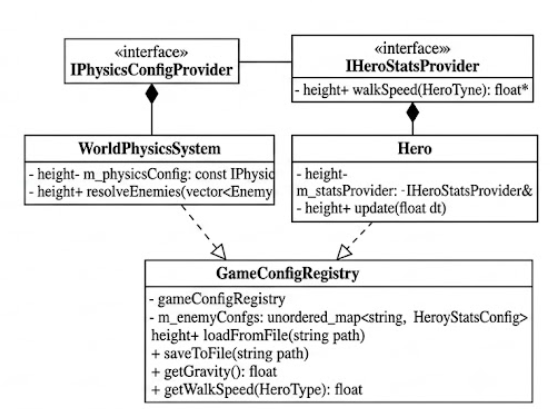
\includegraphics[width=0.45\textwidth]{img/future_suggestion_2.png}
\caption{Proposed Architecture for Data-Driven Gameplay Configuration}
\end{figure}
\section{Project Demonstration}

Due to the dynamic nature of the game engine, real-time mechanics, and audio subsystems, static images cannot fully capture the gameplay experience. Therefore, a comprehensive gameplay demonstration has been recorded and published on YouTube to showcase the integration of our core systems in action.

\subsection{Gameplay Walkthrough}
The demonstration video covers the following key engineering and gameplay features:
\begin{itemize}
    \item \textbf{Initialization and Persistence:} Loading a saved game state using the JSON Save/Load mechanism, which accurately restores the hero's form, inventory, and the state of destroyed map blocks.
    \item \textbf{Item Mechanics and Power-Ups:} Interacting with collectible items such as Mushrooms and Fire Flowers to trigger multi-tier hero evolution forms, alongside collecting coins and hitting interactive \texttt{QuestionBlocks}.
    \item \textbf{Pipe Warp Navigation:} Utilizing pipe entrances to seamlessly travel between different sections of the level, demonstrating smooth sub-area transitions and position resets.
    \item \textbf{Hero Special Abilities:} Executing hero-specific special abilities to defeat enemies.
    \item \textbf{Physics and AI Interaction:} Navigating terrain using dynamic gravity acceleration, dual-pass AABB collision snapping, and engaging patrol-based AI enemies (e.g., Goombas and Koopas).
    \item \textbf{Multi-Phase Boss Encounter:} The climactic battle against \textbf{ThorKing} in Level 1-3. The sequence demonstrates spatial boundary locking, localized SFX playback via the \texttt{SoundManager}, and the boss's complex FSM state transitions.
    \item \textbf{Real-Time UI Integration:} The \texttt{HUDManager} interfacing with the \texttt{PlayingState} to dynamically display and update score, coins, lives, and the remaining time.
\end{itemize}

\subsection{Video Link}
To view the full gameplay recording and system demonstration, please access the link below:

\begin{center}
\url{https://www.youtube.com/watch?v=3uOq83P2HQk}
\end{center}
\section{Conclusion}

The \textbf{Mario Game Project} successfully demonstrates the end-to-end architectural design, mathematical modeling, and software engineering of a fully featured 2D platformer engine developed in C++ using the SFML multimedia framework. Inspired by the foundational mechanics of classic side-scrolling platformers, the system integrates complex gameplay systems—including multi-hero selection (Mario, Luigi, and Flash), multi-tier character evolution (Small, Giant, and Tier-3 Special forms), dynamic AABB collision kinematics, custom artificial intelligence, Tiled map level parsing, spatial partitioning, interactive world elements, HUD metrics, contextual audio streams, and JSON-driven game state persistence.

\subsection{Architectural Achievements and Design Integrity}
A core objective of this project was applying Object-Oriented Programming (OOP) principles and architectural design patterns to resolve the inherent complexity of real-time interactive software. The application of these methodologies yielded substantial benefits across the codebase:
\begin{itemize}
    \item \textbf{Encapsulation and Separation of Concerns:} By strictly decoupling the core render loop (\texttt{GameLoop}), physics mechanics (\texttt{WorldPhysicsSystem}), presentation components (\texttt{HUD}, \texttt{SoundManager}), and world state management (\texttt{LevelRuntime}), individual subsystems were built and maintained independently without propagating collateral bug regressions.
    \item \textbf{Polymorphism and Behavioral Patterns:} The \textit{State/Strategy Pattern} was successfully leveraged to govern hero state transitions and dynamic texture routing without violating the Open/Closed Principle (OCP). The \textit{Factory Pattern} abstracted entity instantiation during map loading, allowing new blocks, items, and character classes to be introduced seamlessly. The \textit{Observer Pattern} cleanly decoupled engine event processing from real-time HUD rendering updates, while the \textit{Template Method Pattern} established reusable patrol and decision-making skeletons for enemy dynamic behavior hierarchies.
\end{itemize}

\subsection{Engineering Bottlenecks and Solutions}
Throughout the development lifecycle, overcoming real-world technical bottlenecks provided deep practical insight into graphics rendering, continuous collision detection, numerical mechanics, and persistent serialization:
\begin{itemize}
    \item \textbf{Mathematical Origin Alignment:} Formulated an automated pixel-alpha Center-of-Mass (CM) padding algorithm to eliminate horizontal sprite jittering and state transition sliding across non-uniform character asset sheets.
    \item \textbf{Kinematic Decoupling in FSM:} Redesigned locomotion state guards by constructing composite input-velocity invariants, permanently resolving high-frequency Finite State Machine (FSM) state oscillations and frame-freezing defects.
    \item \textbf{Map-Agnostic Dynamic Physics:} Replaced fragile hardcoded ground assumptions with continuous dynamic gravity acceleration and dual-pass AABB spatial snapping within \texttt{World\-Physics\-System}, ensuring robust interaction across arbitrary topographies.
    \item \textbf{State Serialization Pipeline:} Architected a deterministic base-reload and JSON overlay mechanism in \texttt{SaveManager}, successfully preserving dynamic entity states, damaged block topologies, player progress metrics, and invulnerability timers.
    \item \textbf{Dynamic Spatial Partitioning:} Implemented context-aware \texttt{PlayableRegion} bounding zones that dynamically clamp camera viewports, eliminate visual border bleeding, adjust underground kill-planes, and switch environmental theme palettes and audio tracks seamlessly.
\end{itemize}

\subsection{Team Synergy and Technical Growth}
The successful completion of the project is attributed to structured collaboration and a clear division of responsibilities among all four team members—spanning Core Engine \& Physics (Tran Minh Khoa), Hero \& Item Mechanics (Tran Nhu Khai), Enemy AI Subsystems (Do Viet Hoang Long), and Level Parsing, UI/UX \& Audio (Tran Dang Khoa). Cooperative version control via Git, structured peer code reviews, and continuous integration testing ensured overall system stability and code consistency throughout the development cycle.

In summary, the Mario Game Project stands as a robust, highly extensible, and production-ready C++ software system. Beyond delivering a smooth and interactive gameplay experience, the project successfully bridged theoretical computer science principles—such as OOP design patterns, state machines, numerical physics simulation, and spatial partitioning—with practical, real-world software architecture.

\pagebreak
\setcounter{page}{1}


\end{document}